\documentclass{beamer}
\usetheme[subsectionpage=progressbar,block=fill]{metropolis}

\definecolor{freifunk-magenta}{rgb}{0.74, 0, 0.35}
%\definecolor{freifunk-gelb}{rgb}{1, 70.31, 0}
\setbeamercolor{frametitle}{bg=freifunk-magenta}
%\setbeamercolor{progress bar in section page}{fg=freifunk-gelb}

\usepackage{svg}
\usepackage{pdfpages}
\usepackage{ngerman}
\usepackage[utf8]{inputenc}                   % replace by the encoding you are using

\title{Dezentrale Vernetzung über den Dächern}
\date{16.07.2019}
\author{Freifunk Franken}
\begin{document}
	\maketitle
	\begin{frame}{Übersicht}
		\tableofcontents
	\end{frame}

	\section{Hotspots}
	\begin{frame}[plain]{Hotspots in Nürnberg}
		\centering
		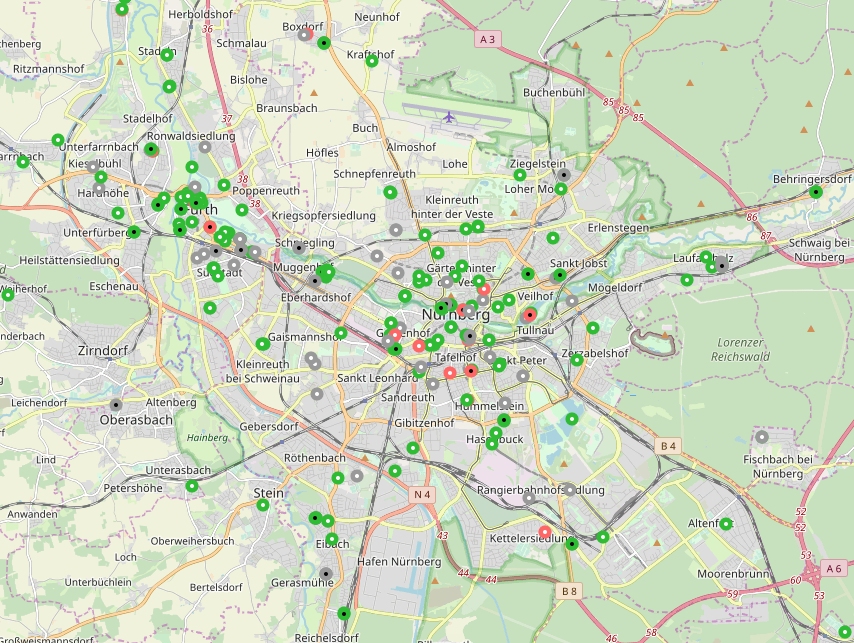
\includegraphics[width=0.94\textwidth]{media/hotspots.png}
	\end{frame}
	\begin{frame}{Freifunk Hotspots}
		\begin{block}{Hotspots}
			\begin{itemize}
				\item Bekannteste Form von Freifunk
				\item Auch in Nürnberg/Franken
			\end{itemize}
		\end{block}
		\vspace{1em}
		\pause
		\begin{block}{Teilen des eigenen Internetanschlusses}
			\begin{itemize}
				\item Router mit Freifunk Firmware
				\item Tunnel zu Freifunk Server
				\item Umgehung rechtlicher Probleme
			\end{itemize}
		\end{block}
	\end{frame}

	\section{Vernetzung per Mesh}
	\begin{frame}{Vernetzen per Mesh}
		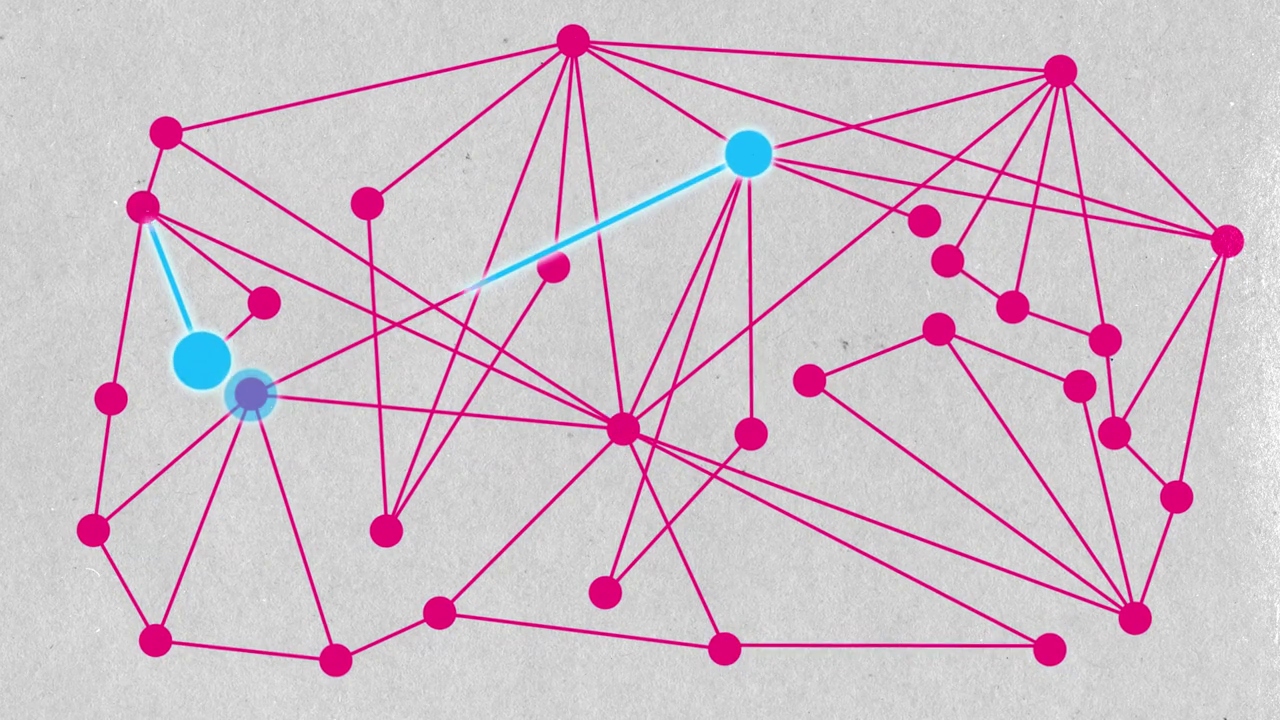
\includegraphics[width=\textwidth]{media/mesh2.png}
	\end{frame}

	%\subsection{Entwicklung}
% 	\begin{frame}{Entwicklung}
% % "wie man sich mesh vorgestellt hat" stattdessen
% 		\begin{block}{Hotspots}
% 			\begin{itemize}
% 				\item Immer mehr
% 				\item Teilweise in Kooperation mit Städten
% 			\end{itemize}
% 		\end{block}
% 		\vspace{1em}
% 		\pause
% 		\begin{block}{Backend}
% 			\begin{itemize}
% 				\item Wenig Interaktion zwischen Freifunkern
% 				\item Mesh eher selten und extrem langsam
% 				\item Klappt nicht so, wie man sich das dachte
% 			\end{itemize}
% 		\end{block}
% 	\end{frame}

% wlan frequenzen, belegung, überscheidung
% doppelt verbrauchte airtime animation
% multicasts werden langsam gesendet
% jeder sieht jeden

	{
		\setbeamercolor{background canvas}{bg=}
		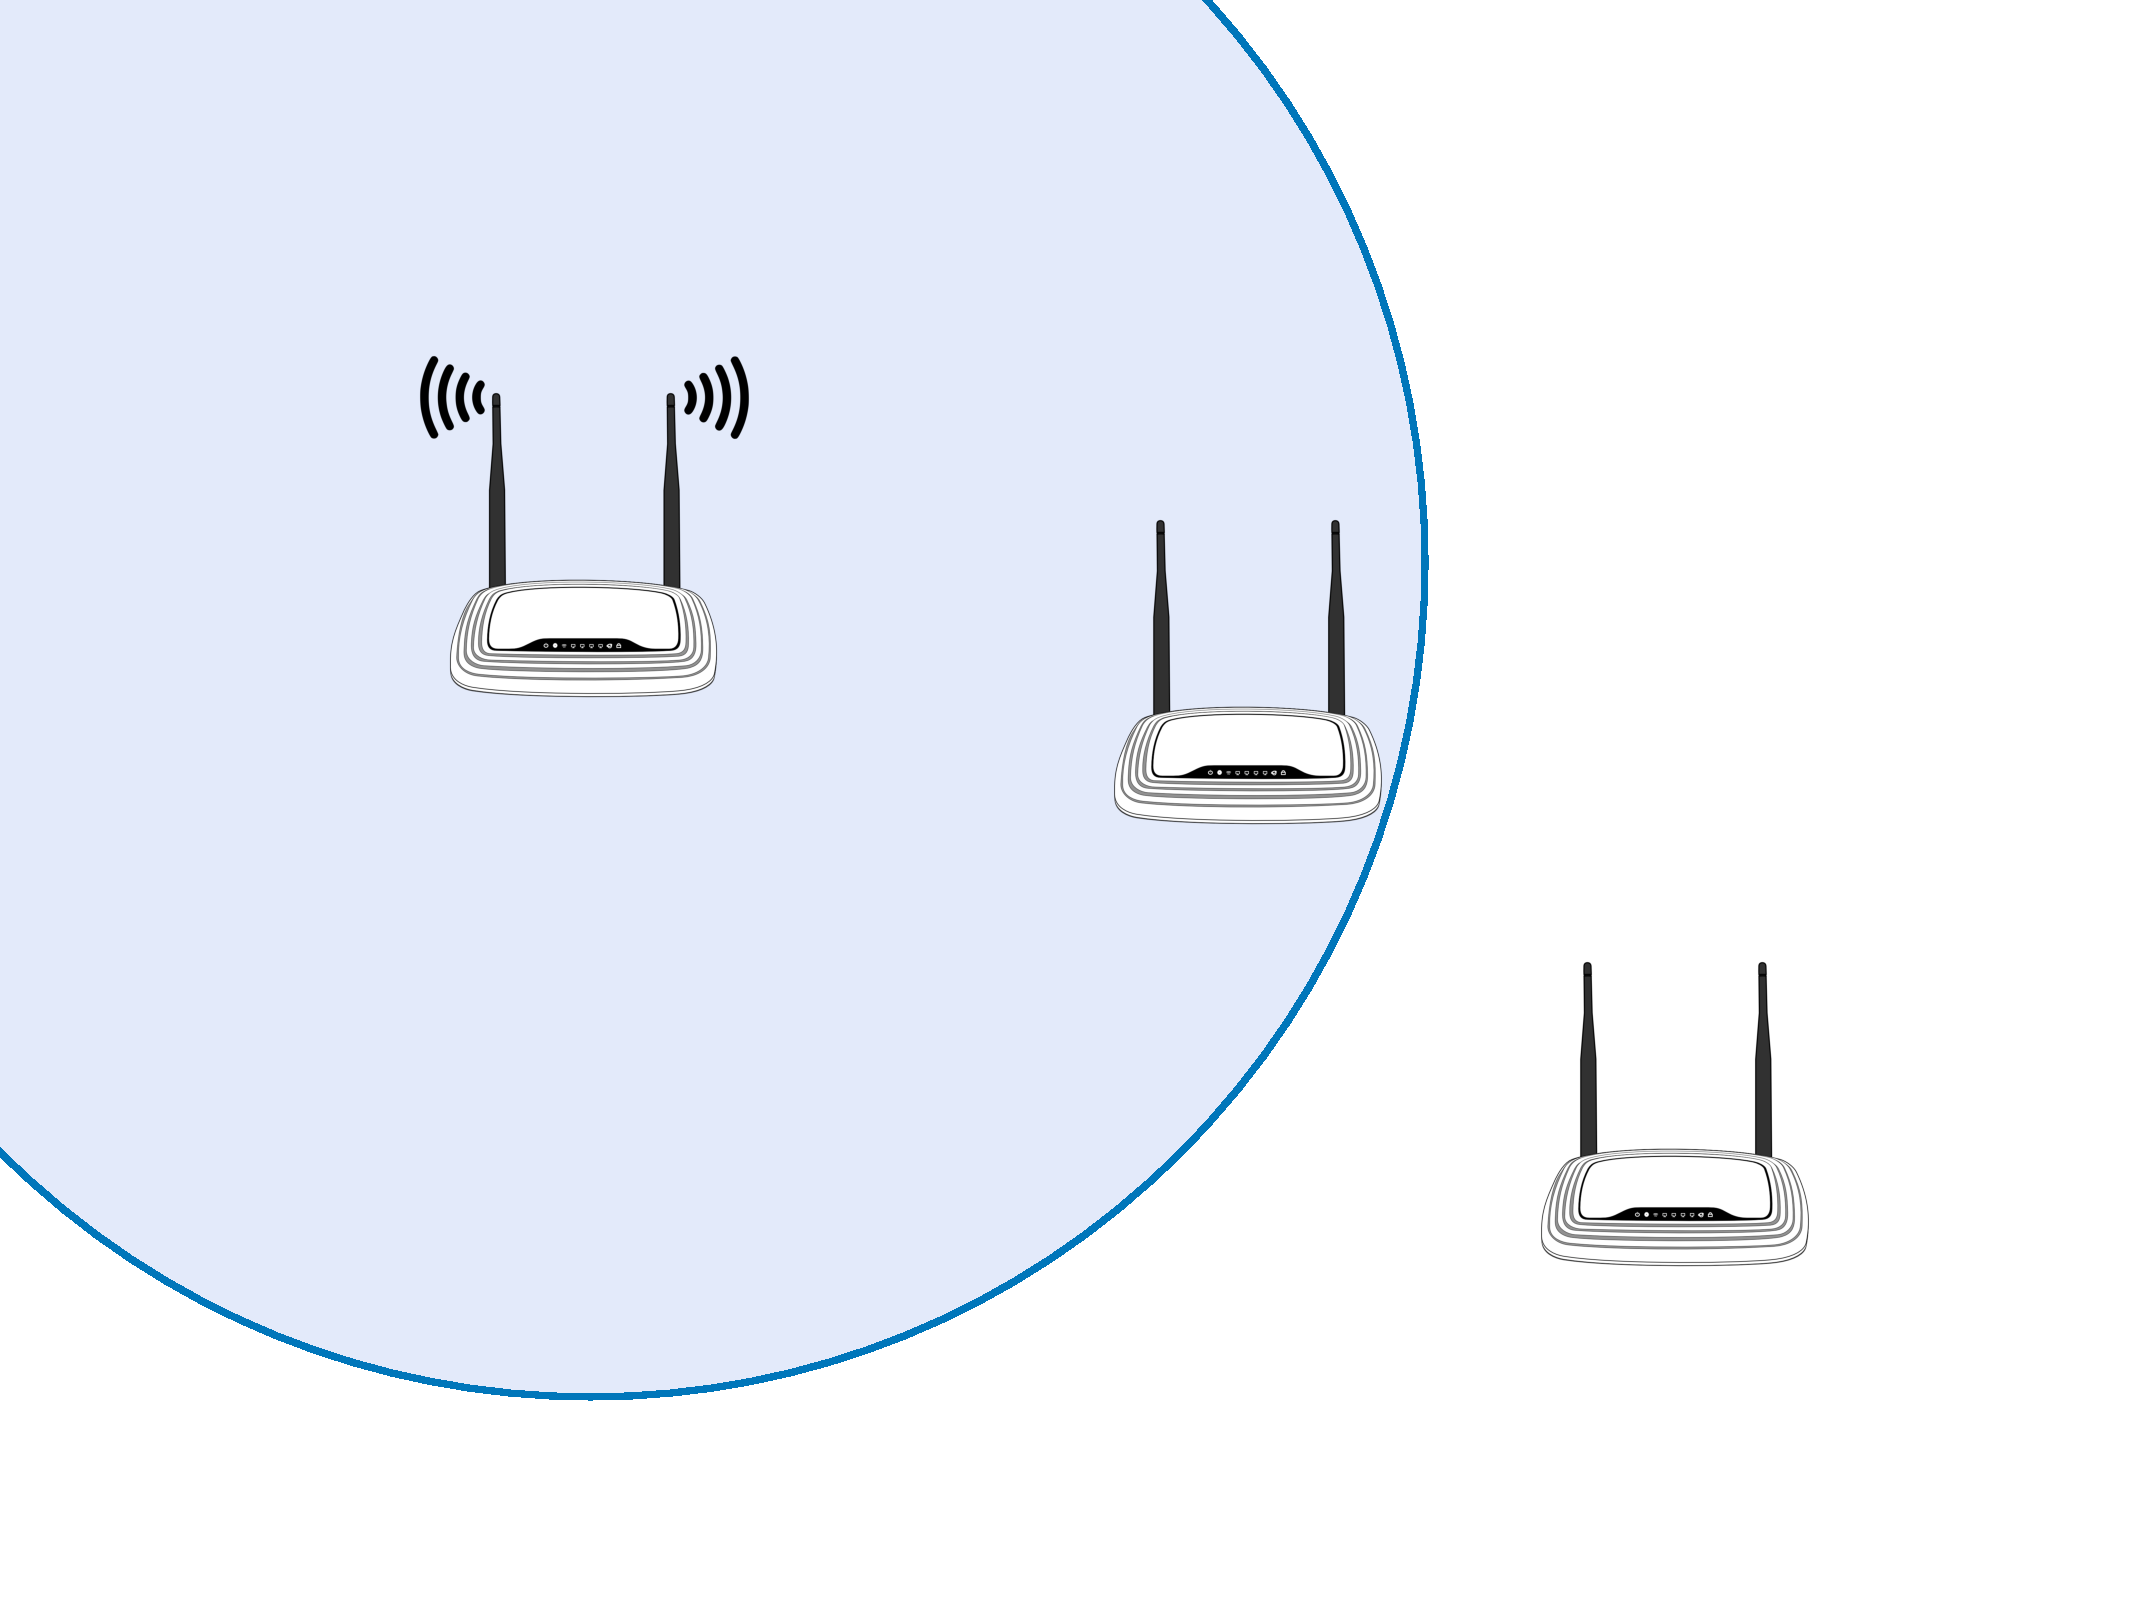
\includepdf[pages=1-11]{media/animation.pdf}
	}

	\subsection{Doppelt verbrauchte Luft}
	{
		\setbeamercolor{background canvas}{bg=}
		\includepdf[pages=12-16]{media/animation.pdf}
	}

	\subsection{Broadcasts}
	{
		\setbeamercolor{background canvas}{bg=}
		\includepdf[pages=17-21]{media/animation.pdf}
	}

	\subsection{Hidden Nodes}
	{
		\setbeamercolor{background canvas}{bg=}
		\includepdf[pages=22-27]{media/animation.pdf}
	}

	\begin{frame}{Mesh skaliert nicht!}
	\begin{block}{technisch}
		\begin{itemize}
			\item Begrenzte Frequenzen
			\item Mehrfach verbrauchte Airtime
			\item Zu viel nutzloser Broadcast
			\item Dedizierter Firmware/Hardware notwendig
		\end{itemize}

	\end{block}
	\begin{block}{sozial}
		\begin{itemize}
			\item wenig Interaktion nötig
			\begin{itemize}
			 \item[$\rightarrow$] wenig Interaktion zwischen Freifunkern
			\end{itemize}

		\end{itemize}
	\end{block}
	\end{frame}

	\begin{frame}[standout]
		Back to the drawing board!
	\end{frame}

	\begin{frame}{Pico-Peering Agreement}
		\textbf{Regelwerk, über grundsätzliche Eigenschaften des Freifunks}

		\begin{enumerate}
			\item Freier Transit
			\item Offene Kommunikation
			\item Keine Garantie (Haftungsausschluss)
			\item Nutzungsbestimmungen
			\item Lokale (individuelle) Zusätze
		\end{enumerate}
	\end{frame}

	\section{Dezentrale Vernetzung}
	\begin{frame}[plain,standout]
		% Mast von Tobias -> Bilderstrecke auch mit unterschiedlichen Installationsmöglichkeiten?
		%                 -> Fensterbank/Flaschenhalter/Gewächshaus usw.
		% Reichweite (Monitoring Screenshots)
		% Speedtest
		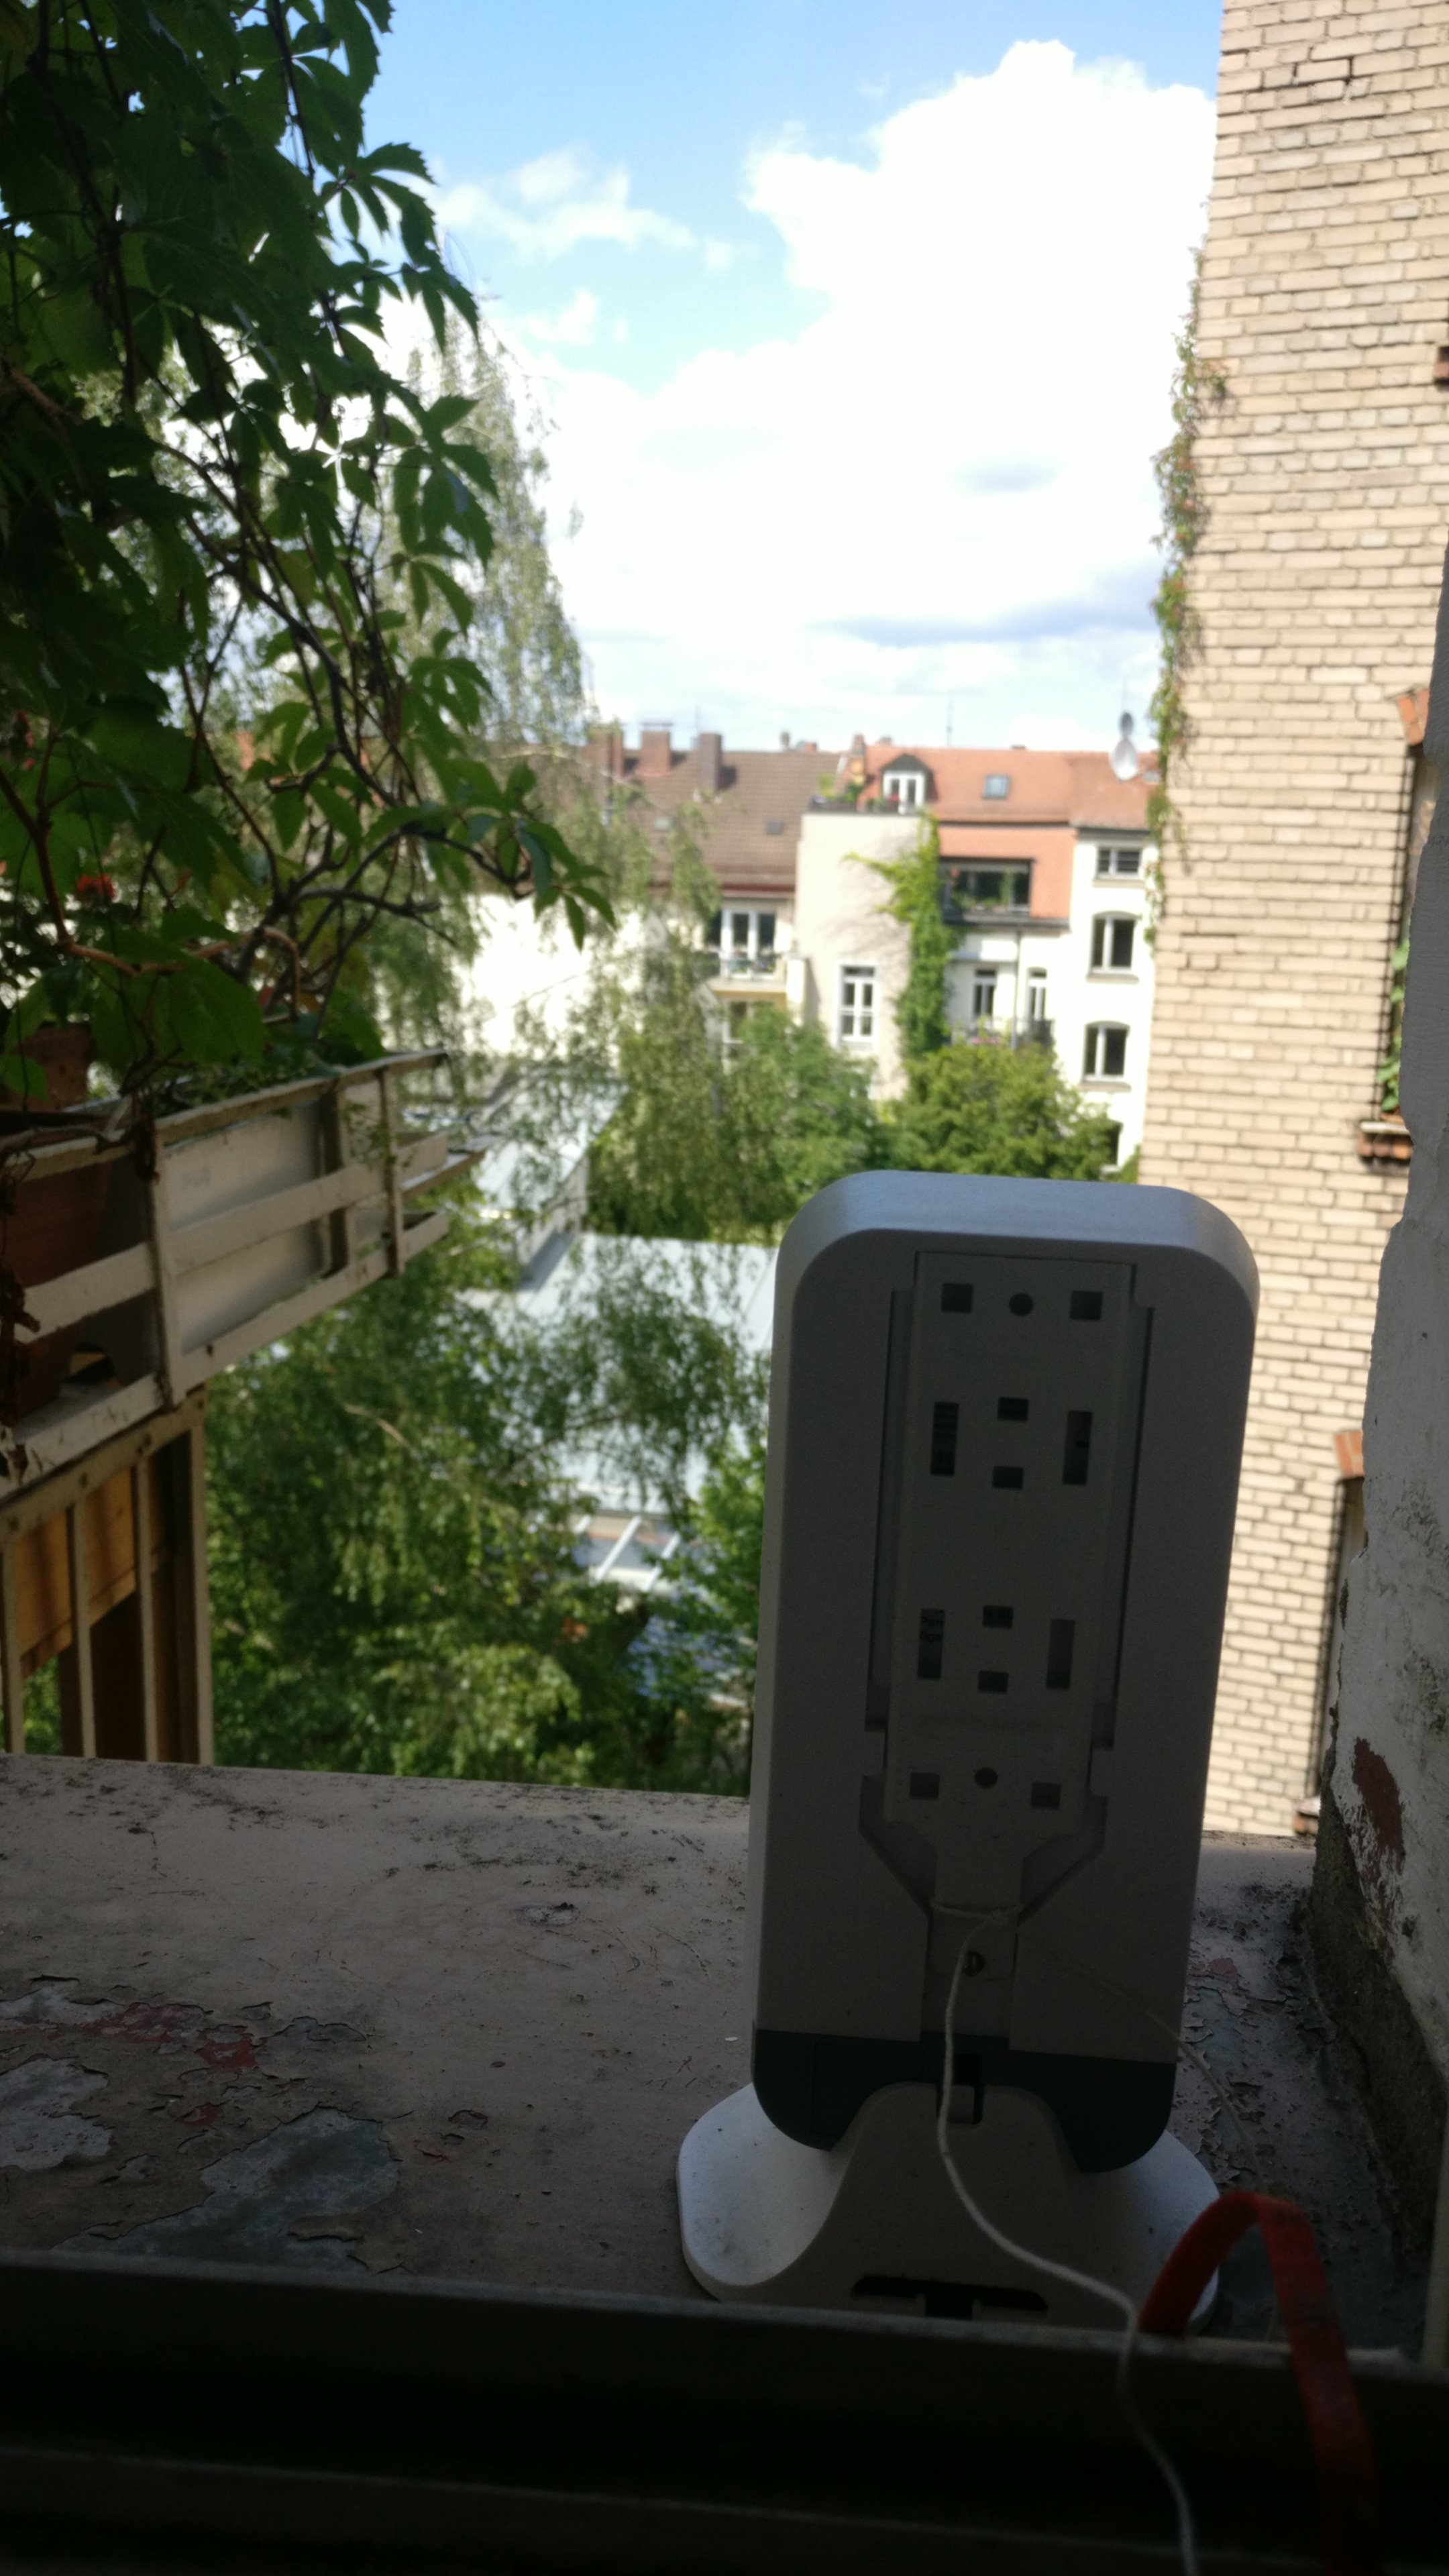
\includegraphics[height=0.75\framewidth]{media/p2p-fensterbrett1.jpg}
	\end{frame}
	\begin{frame}[plain,standout]
		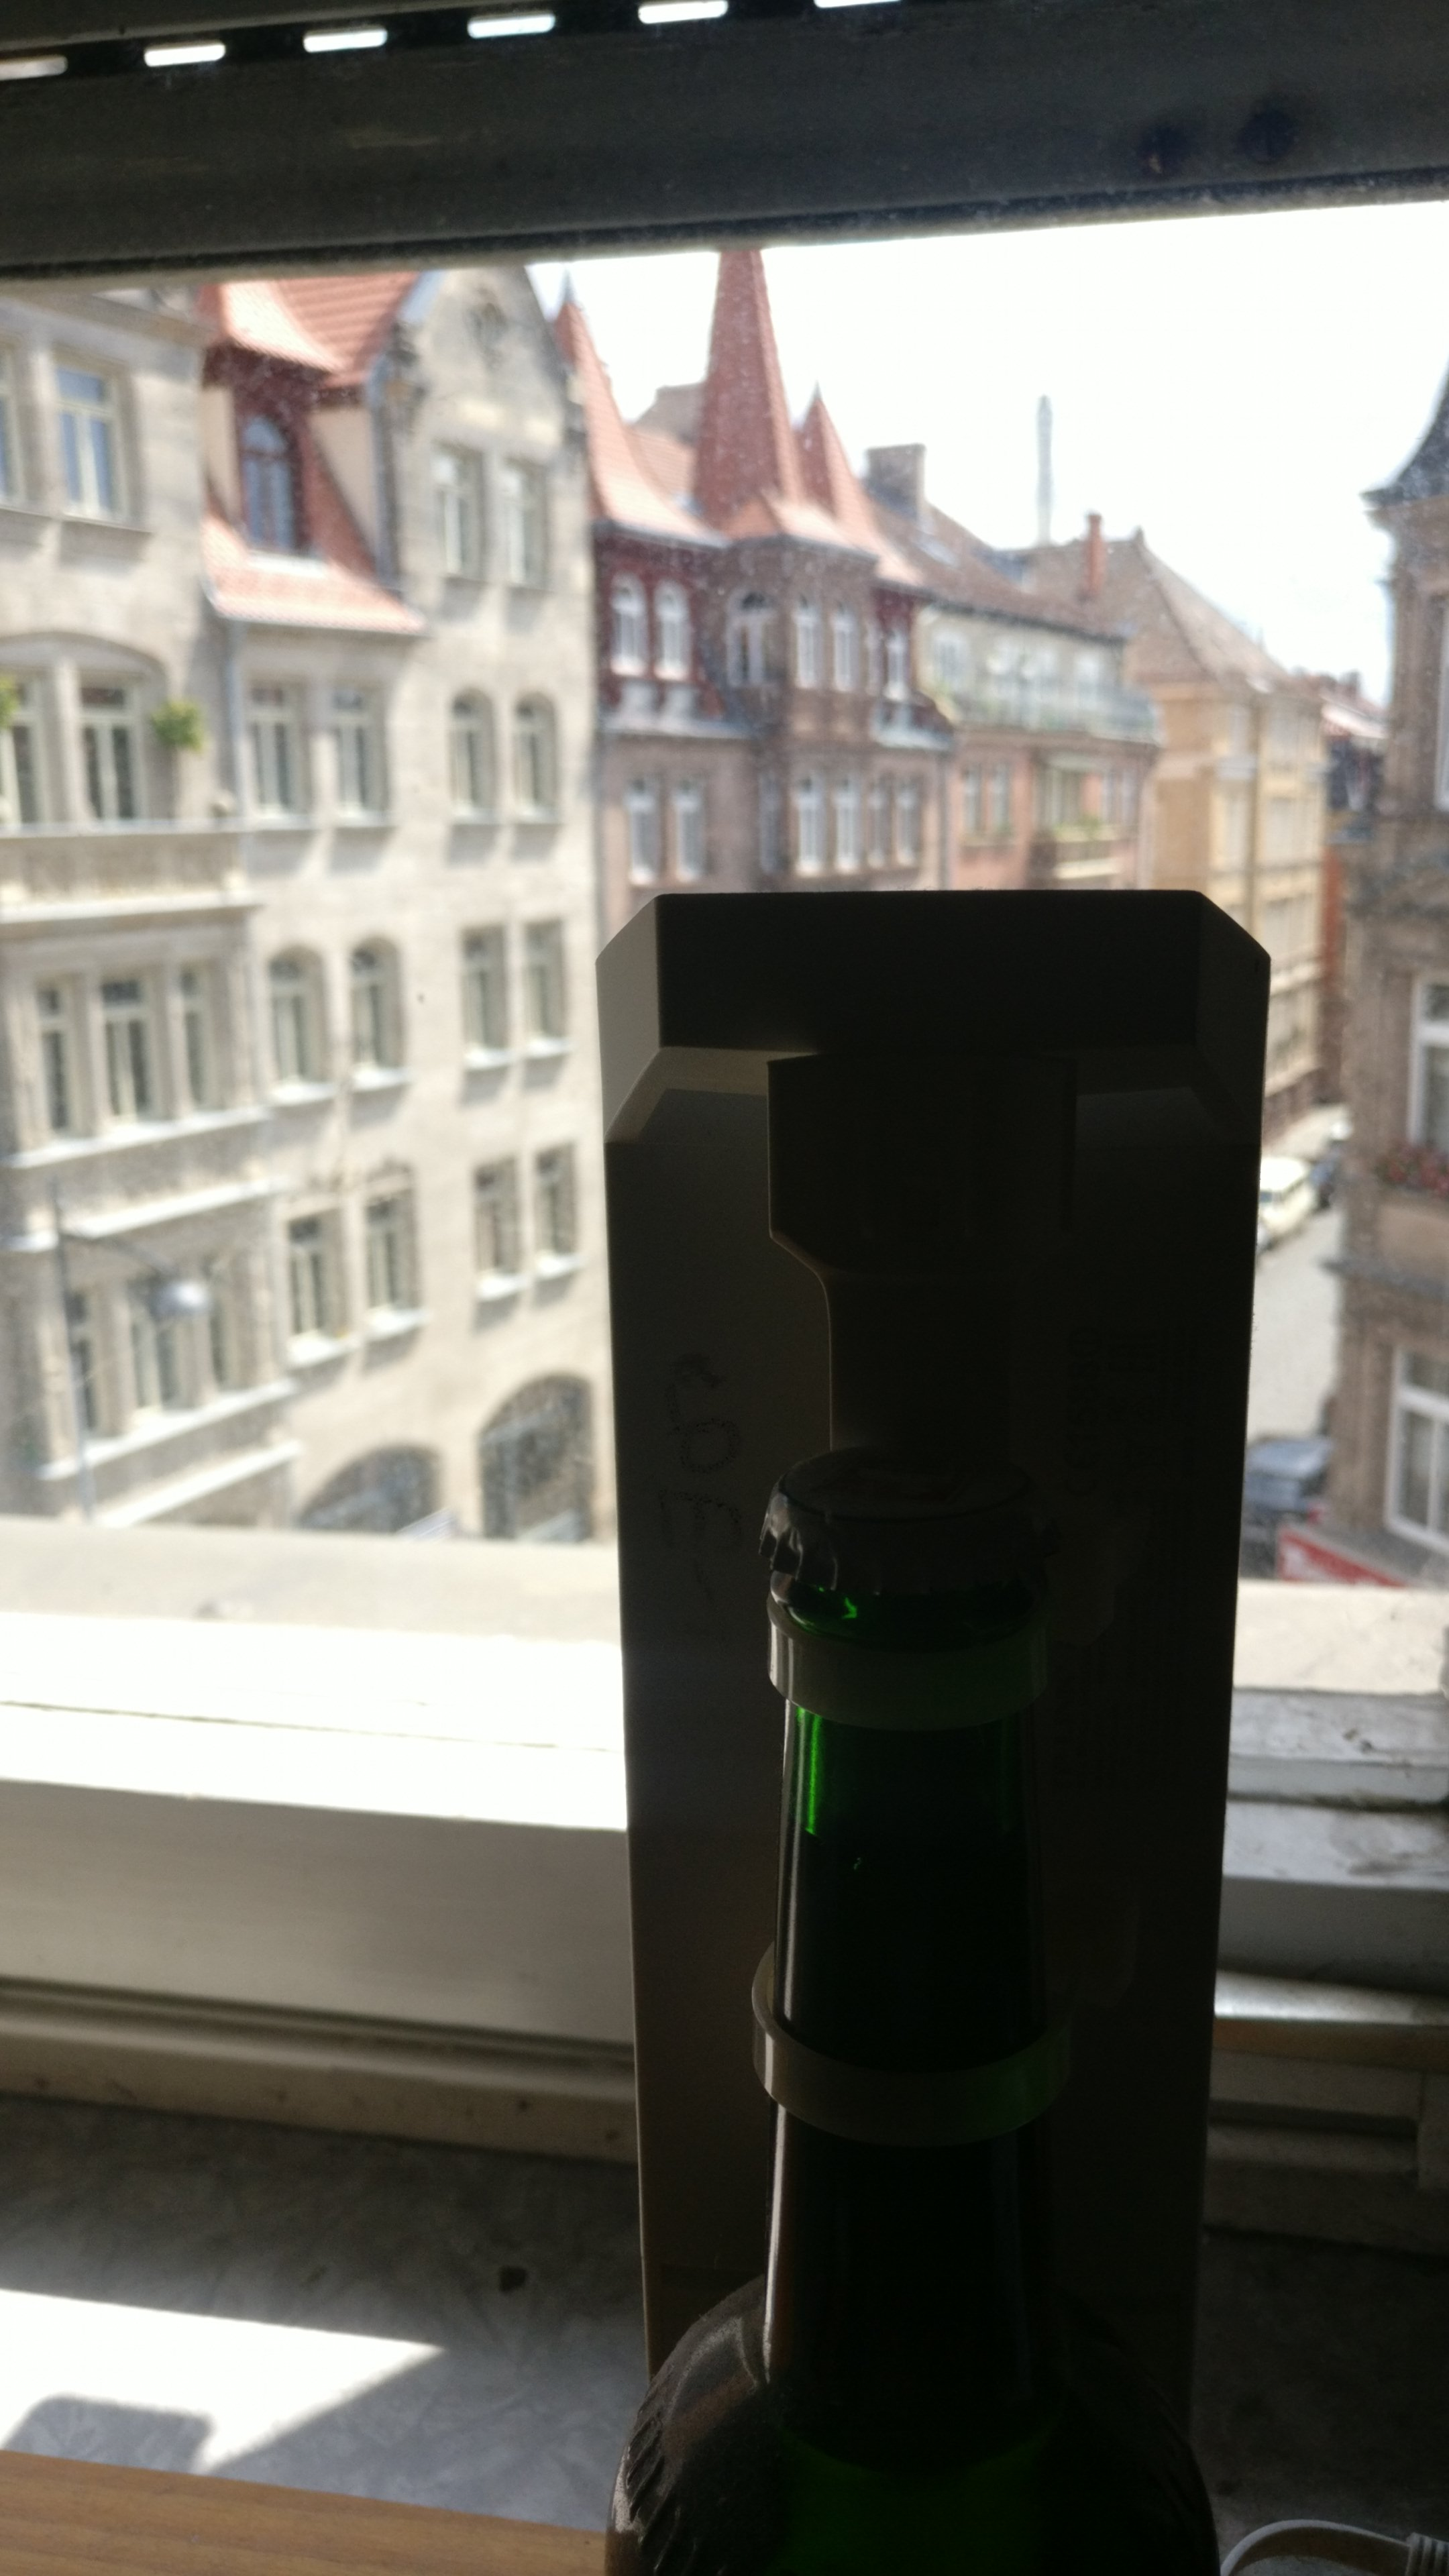
\includegraphics[height=0.75\framewidth]{media/p2p-flasche2.jpg}
	\end{frame}
	\begin{frame}[plain,standout]
		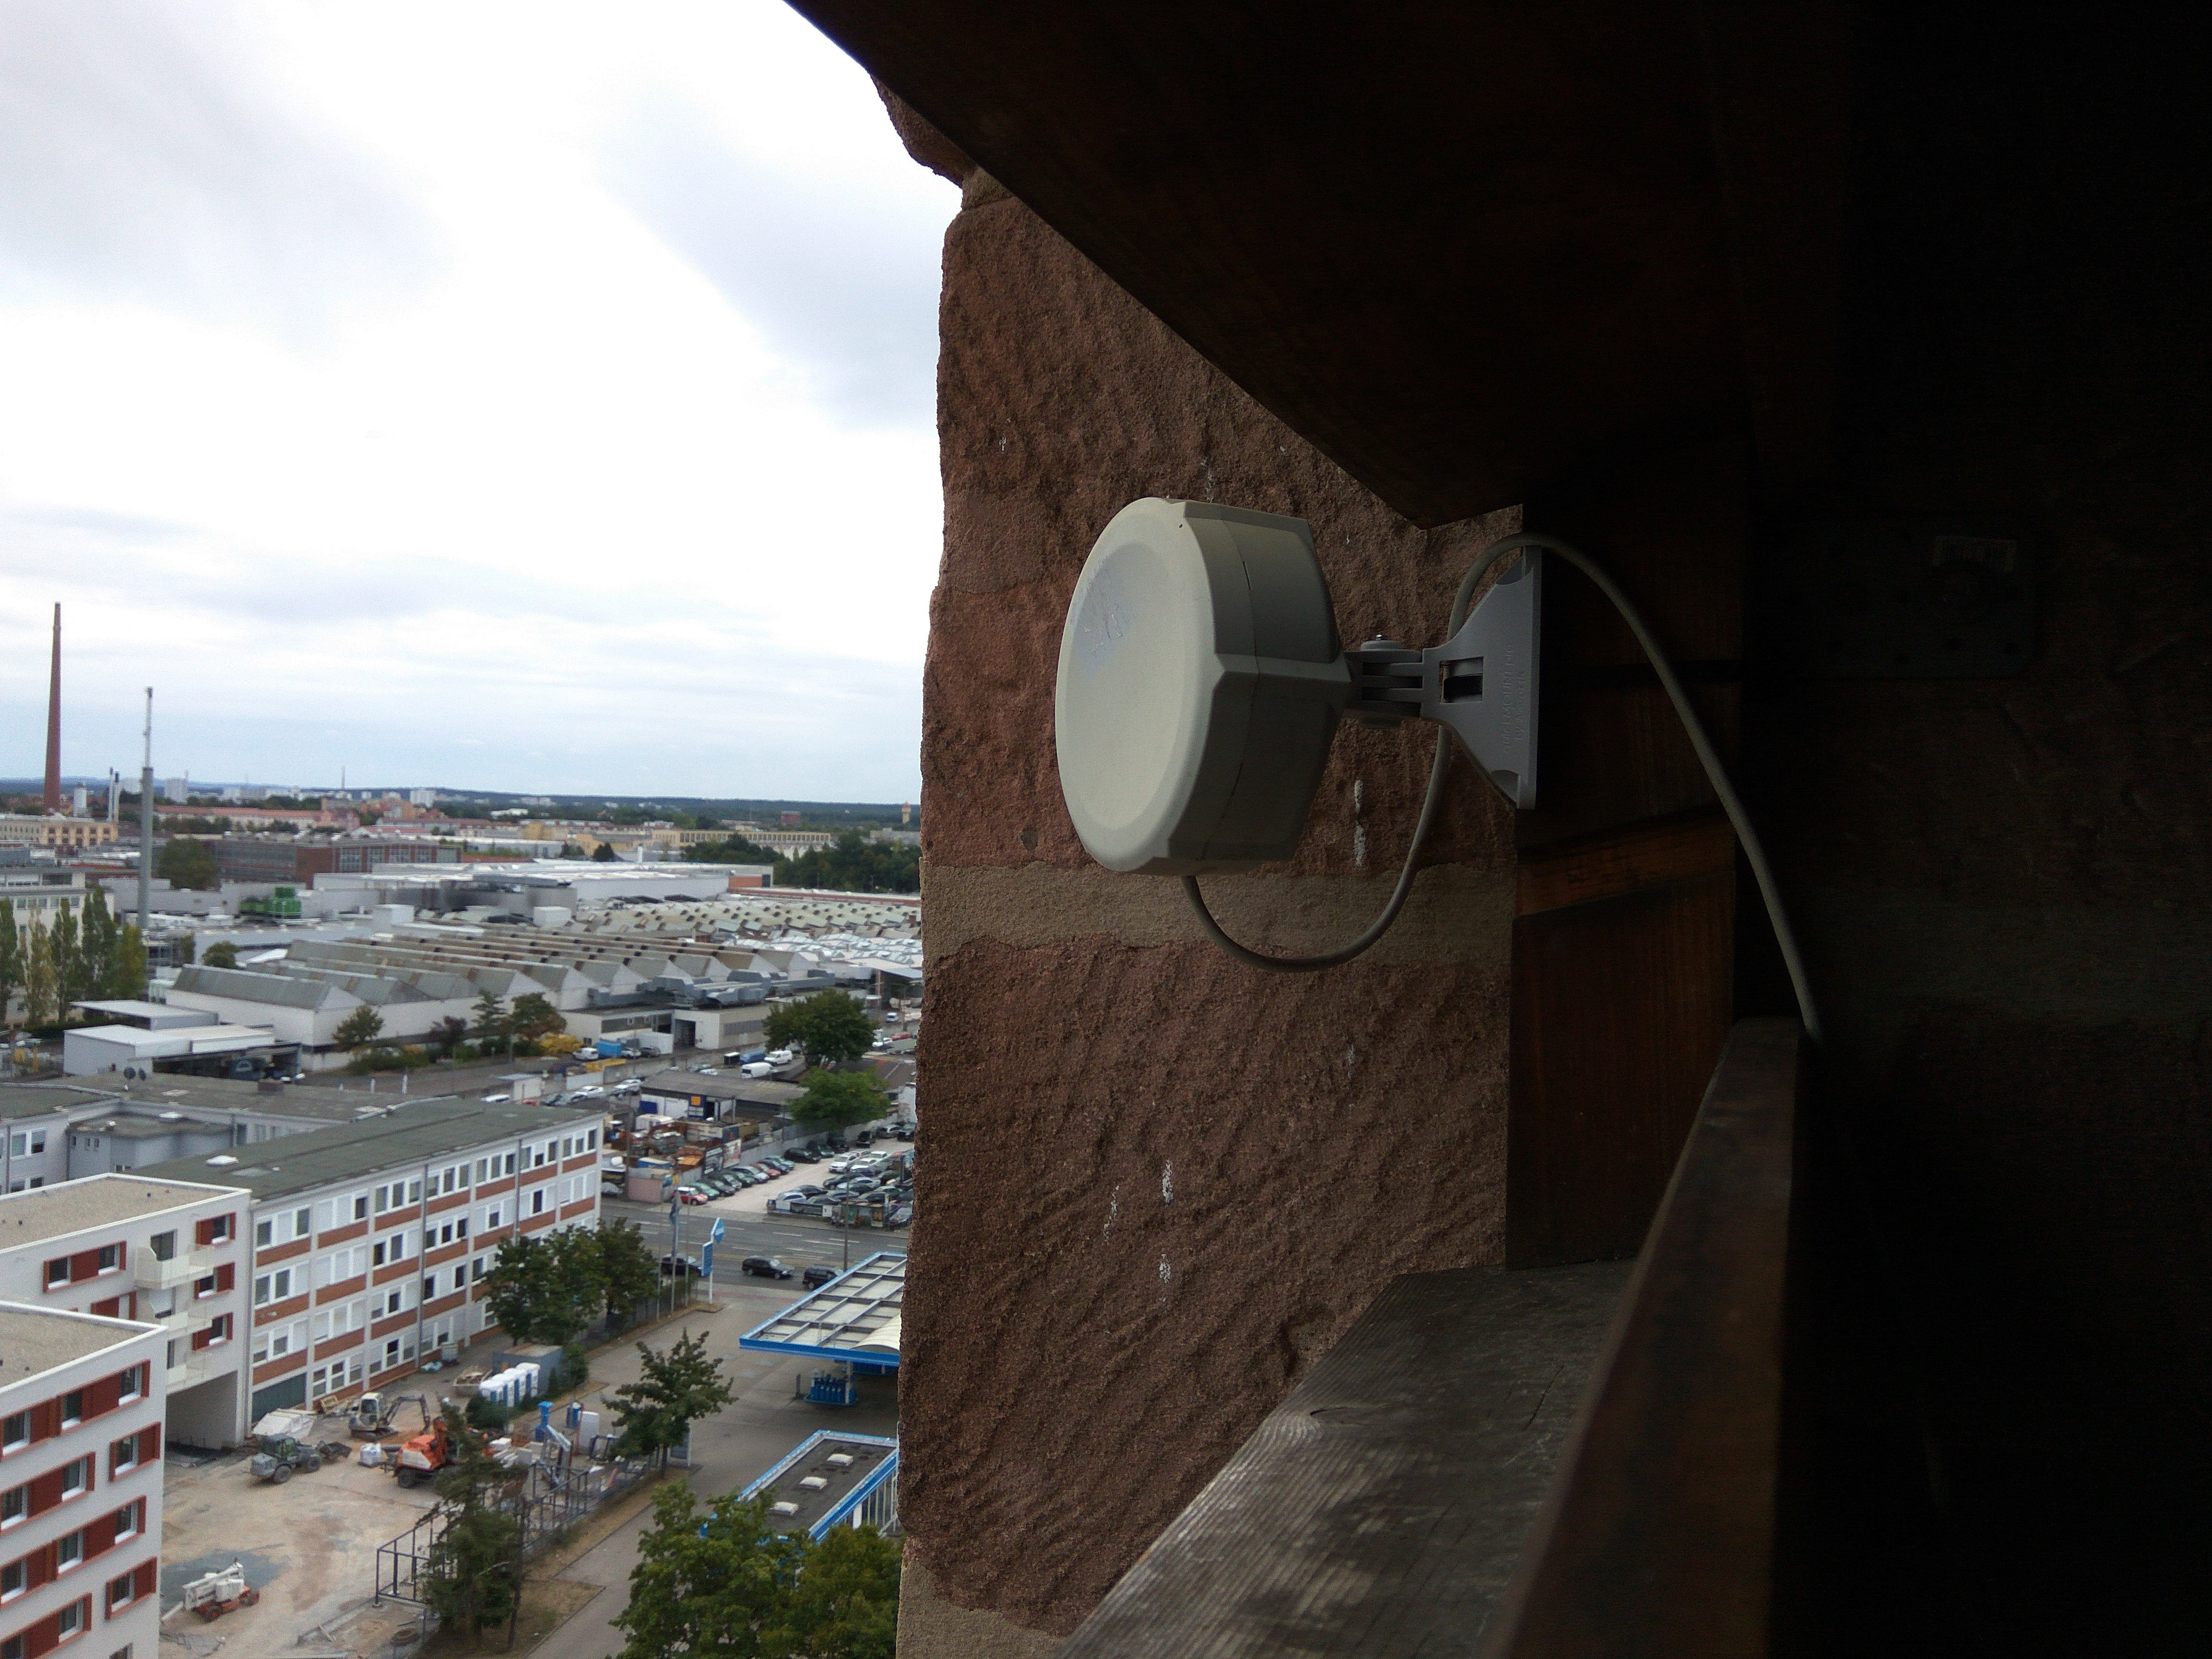
\includegraphics[width=\framewidth]{media/p2p-sxt.jpg}
	\end{frame}
	\begin{frame}[plain,standout]
		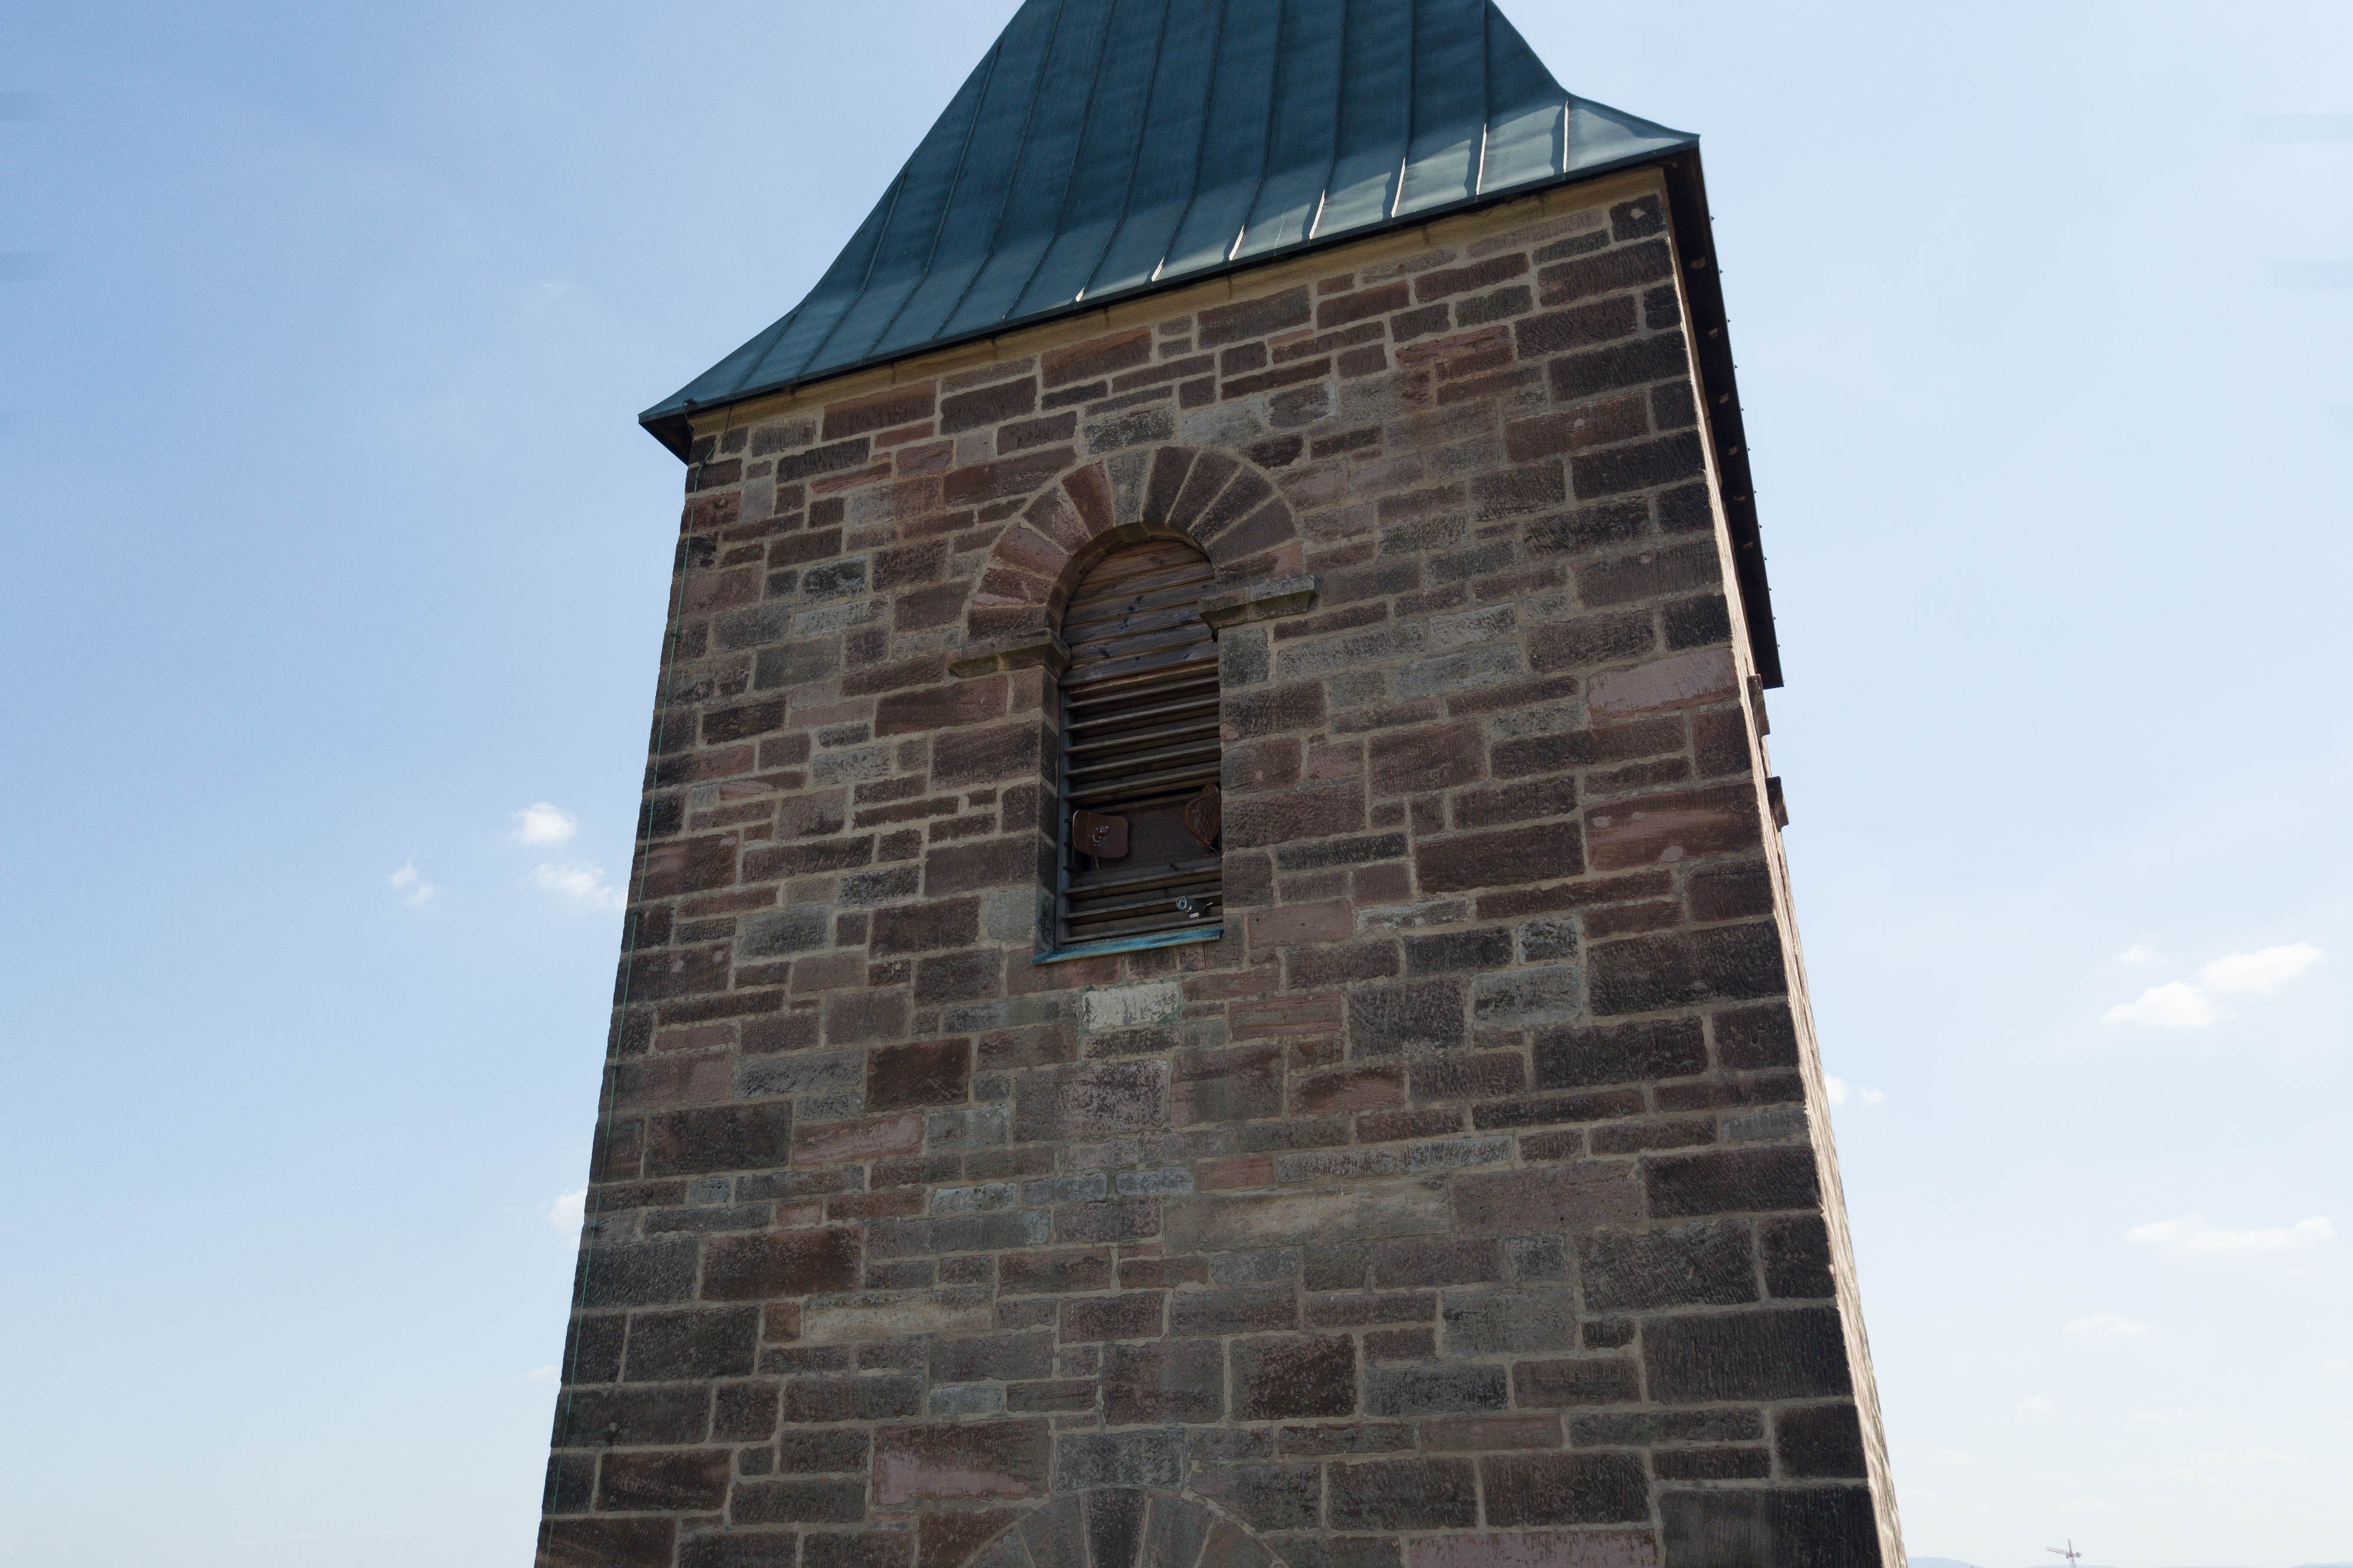
\includegraphics[width=\framewidth]{media/p2p-stmarkus.jpg}
	\end{frame}
	\begin{frame}[plain,standout]
		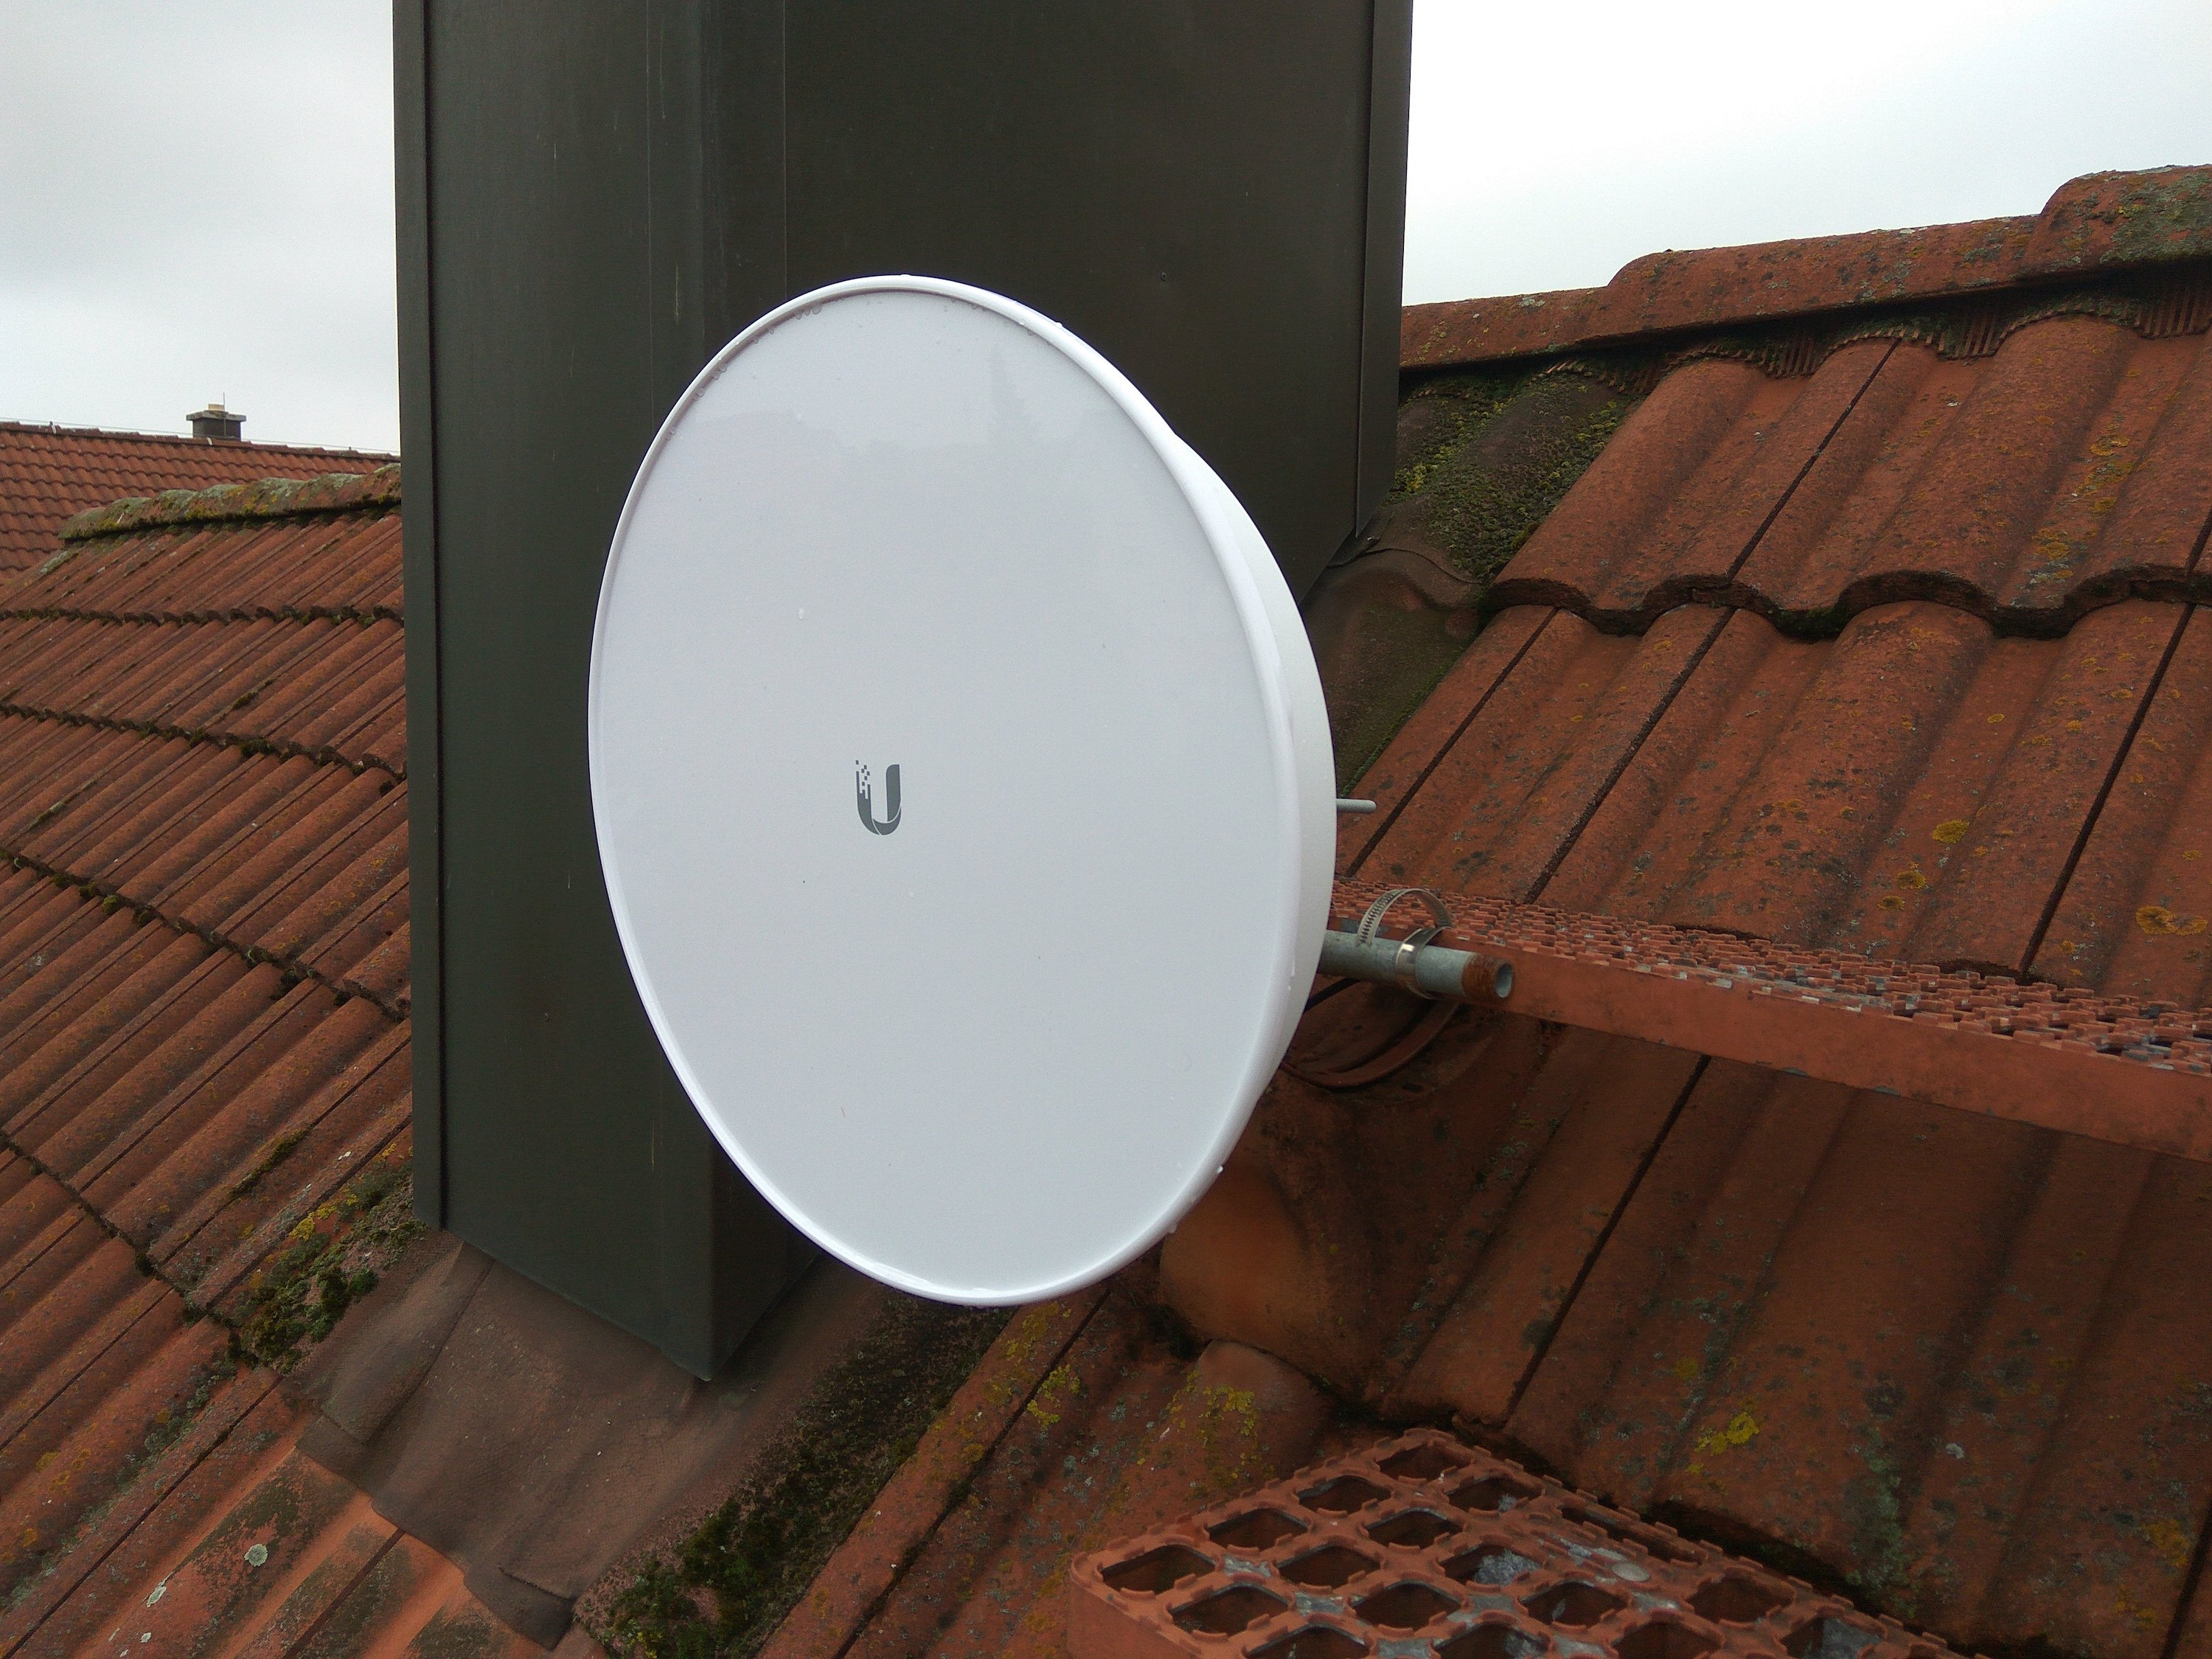
\includegraphics[width=\framewidth]{media/p2p-wohnhaus.jpg}
	\end{frame}
	\begin{frame}[plain,standout]
		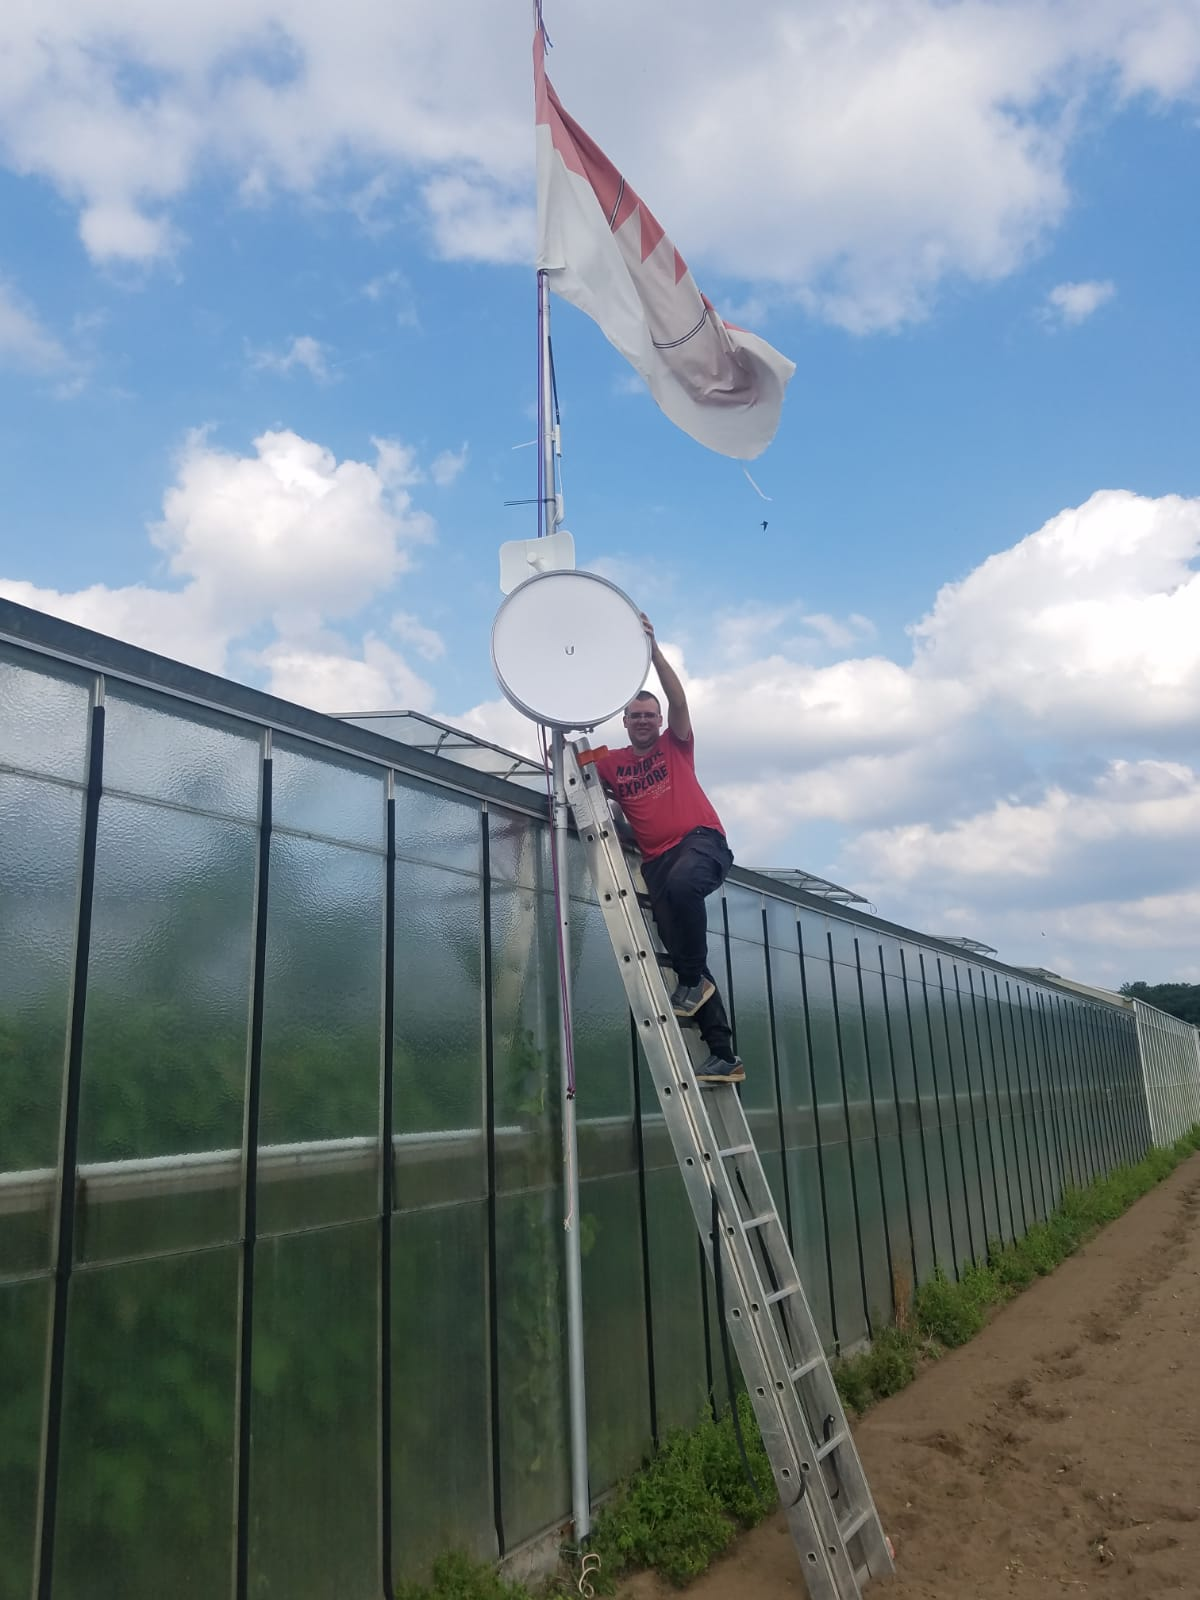
\includegraphics[height=0.75\framewidth]{media/p2p-treibhaus.jpg}
	\end{frame}
	\begin{frame}[plain,standout]
		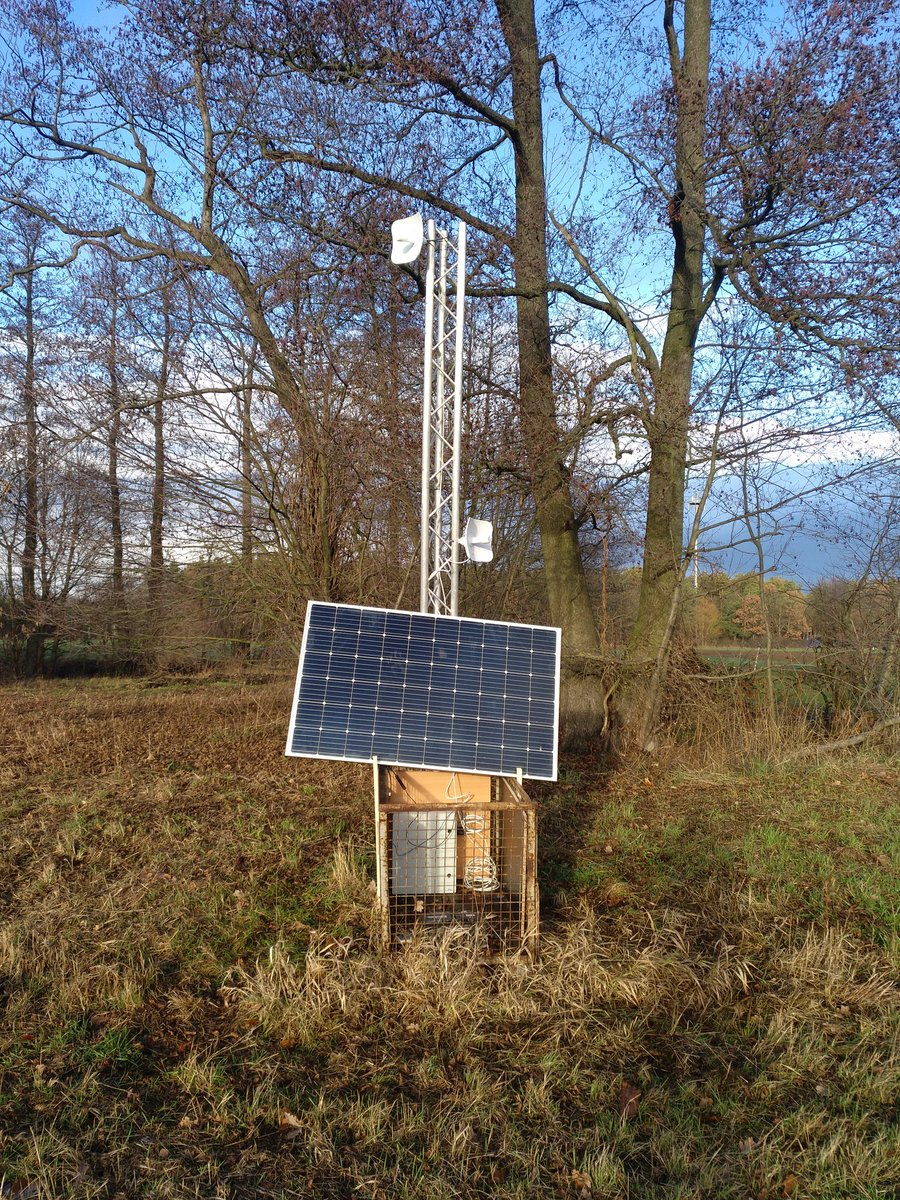
\includegraphics[height=0.75\framewidth]{media/p2p-solar.jpg}
	\end{frame}


	\begin{frame}{Unabhängige Netze}
		% Skalierbar
		% Gewöhnliche Zugangspunkte
		% Kontrolle über eigenes Netz
	\end{frame}
	\begin{frame}{Back to the Roots}
            %was wollten wir hier nochmal machen?
	\end{frame}

	\begin{frame}[plain,standout]
		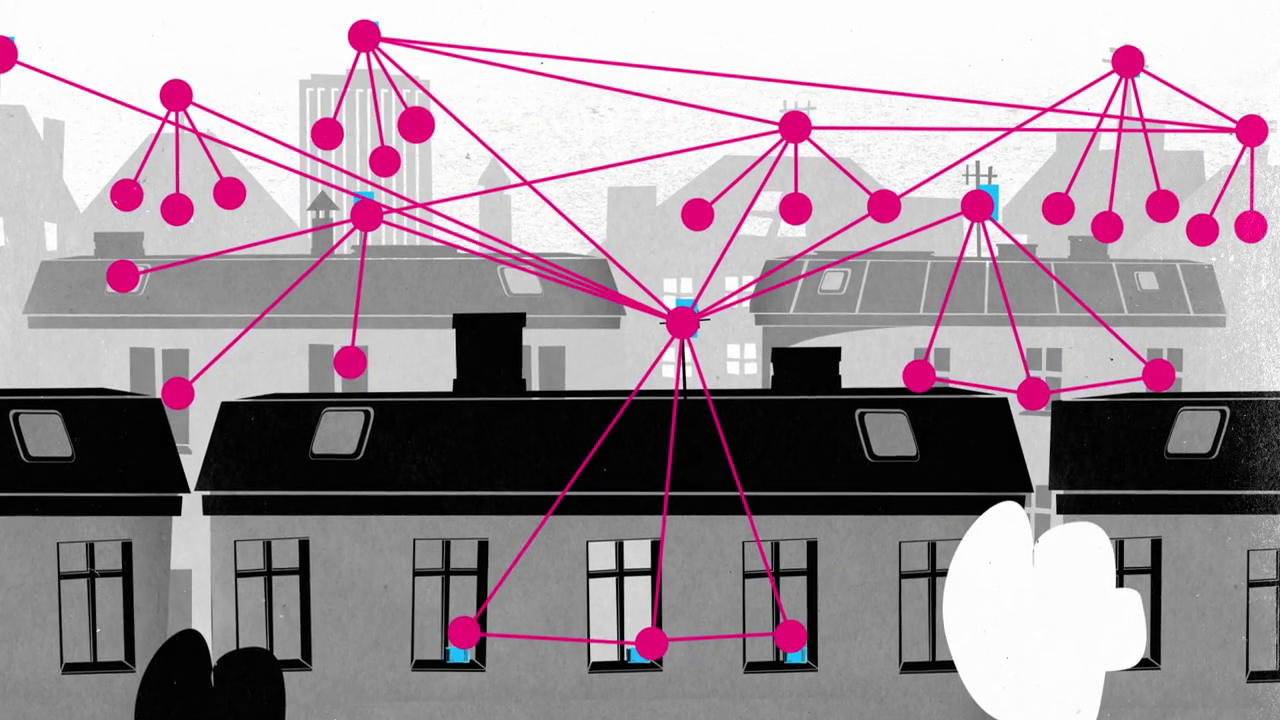
\includegraphics[width=\framewidth]{media/dachzudach.png}
	\end{frame}
	\begin{frame}[plain,standout]
		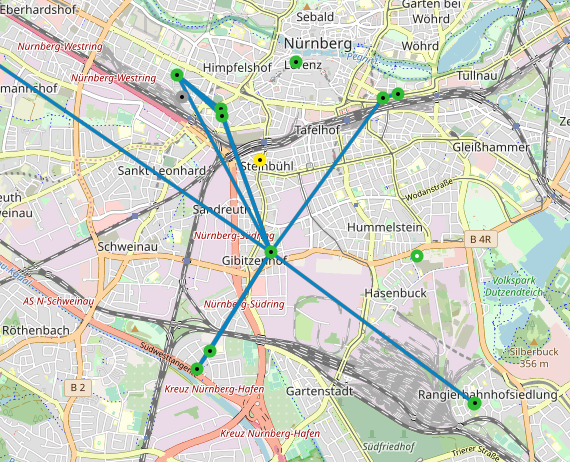
\includegraphics[height=\textheight]{media/rf_nbg.png}
	\end{frame}
	\begin{frame}[plain,standout]
		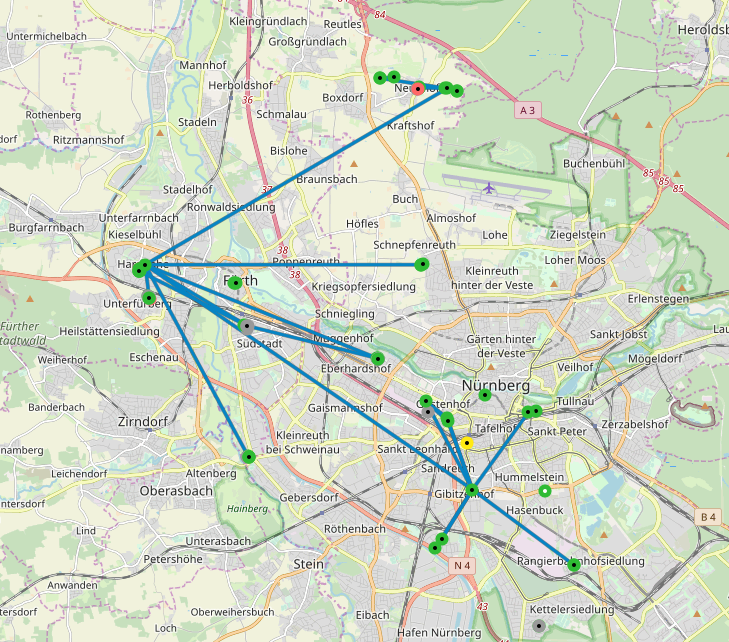
\includegraphics[height=\textheight]{media/rf_nbgfue.png}
	\end{frame}

	\begin{frame}{Zusammenfassung}
		\begin{block}{Gezielte Verbindungen}
		\begin{itemize}
			\item Dedizierte Hardware
			\item Höhere Reichweite
			\item Deutlich höhere Geschwindigkeit
		\end{itemize}
		\end{block}
		\begin{block}{Unabhängige Netze}
		\begin{itemize}
			\item
		\end{itemize}
		\end{block}
		\begin{block}{Etablierte Standards}
		\begin{itemize}
			\item IP-Routing
			\item Standardhardware
			\item Anwendung von bekanntem Wissen
		\end{itemize}
		\end{block}
	\end{frame}

% Exkurs: IPv6
	% Konkrete Vorteile
	%% Public IPv6
	%% Dinge zuhause [sinnvoll] hosten
	%% Erreichbarkeit bestimmter Netze ohne Abhängigkeit von großen ISP
	%%% symmetrische Verbindungen
	\begin{frame}{Exkurs: IPv6}
		\begin{block}{Internet Protocol Version 6}
		\begin{itemize}
			\item Nachfolger von IPv4
			\item $2^{128}$ Adressen
			\item Seit 1998 standardisiert
		\end{itemize}
		\end{block}
		\pause
		\begin{block}{Im Freifunk}
		\begin{itemize}
			\item Öffentliche Adressen
			\item Weltweit erreichbar
			\item Statisch delegiert
			\begin{itemize}
			 \item[$\rightarrow$] Dienste können von zuhause bereitgestellt werden
			\end{itemize}
		\end{itemize}
		\end{block}
	\end{frame}

	\begin{frame}[plain,standout]
		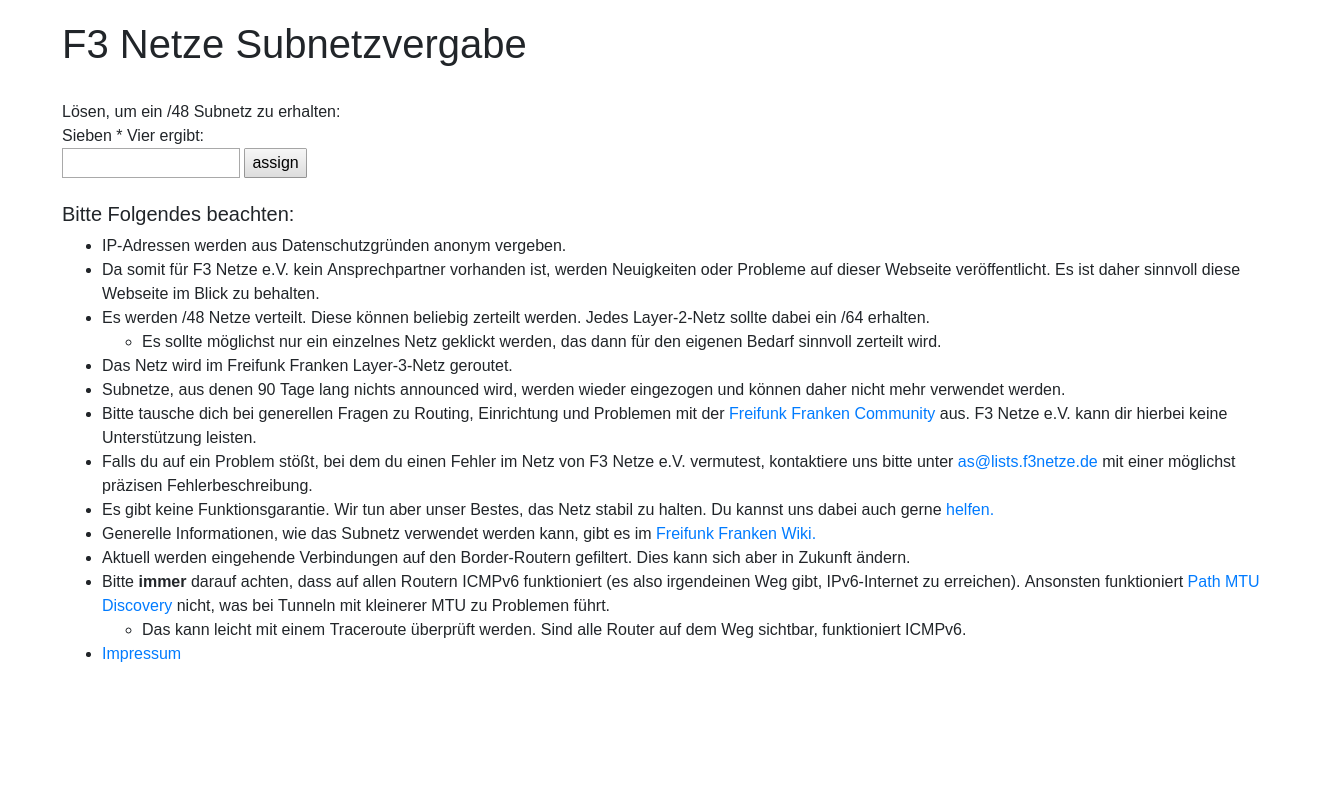
\includegraphics[width=\framewidth]{media/f3nsub.png}
	\end{frame}

% N-IX: Ausblick: Direkte [tunnelfreie] Anbindung ans Internet
	\section{Ausblick}
	\begin{frame}{Eigene Anbindung ans Internet}
		\begin{itemize}
			\item Aktuell Anbindung per Tunnel zu Servern
			\item Mittlerweile eigenes AS
			\item Direkte Verbindung ohne Tunnel zum Internet
		\end{itemize}
	\end{frame}
	\begin{frame}[plain,standout]
		\centering
		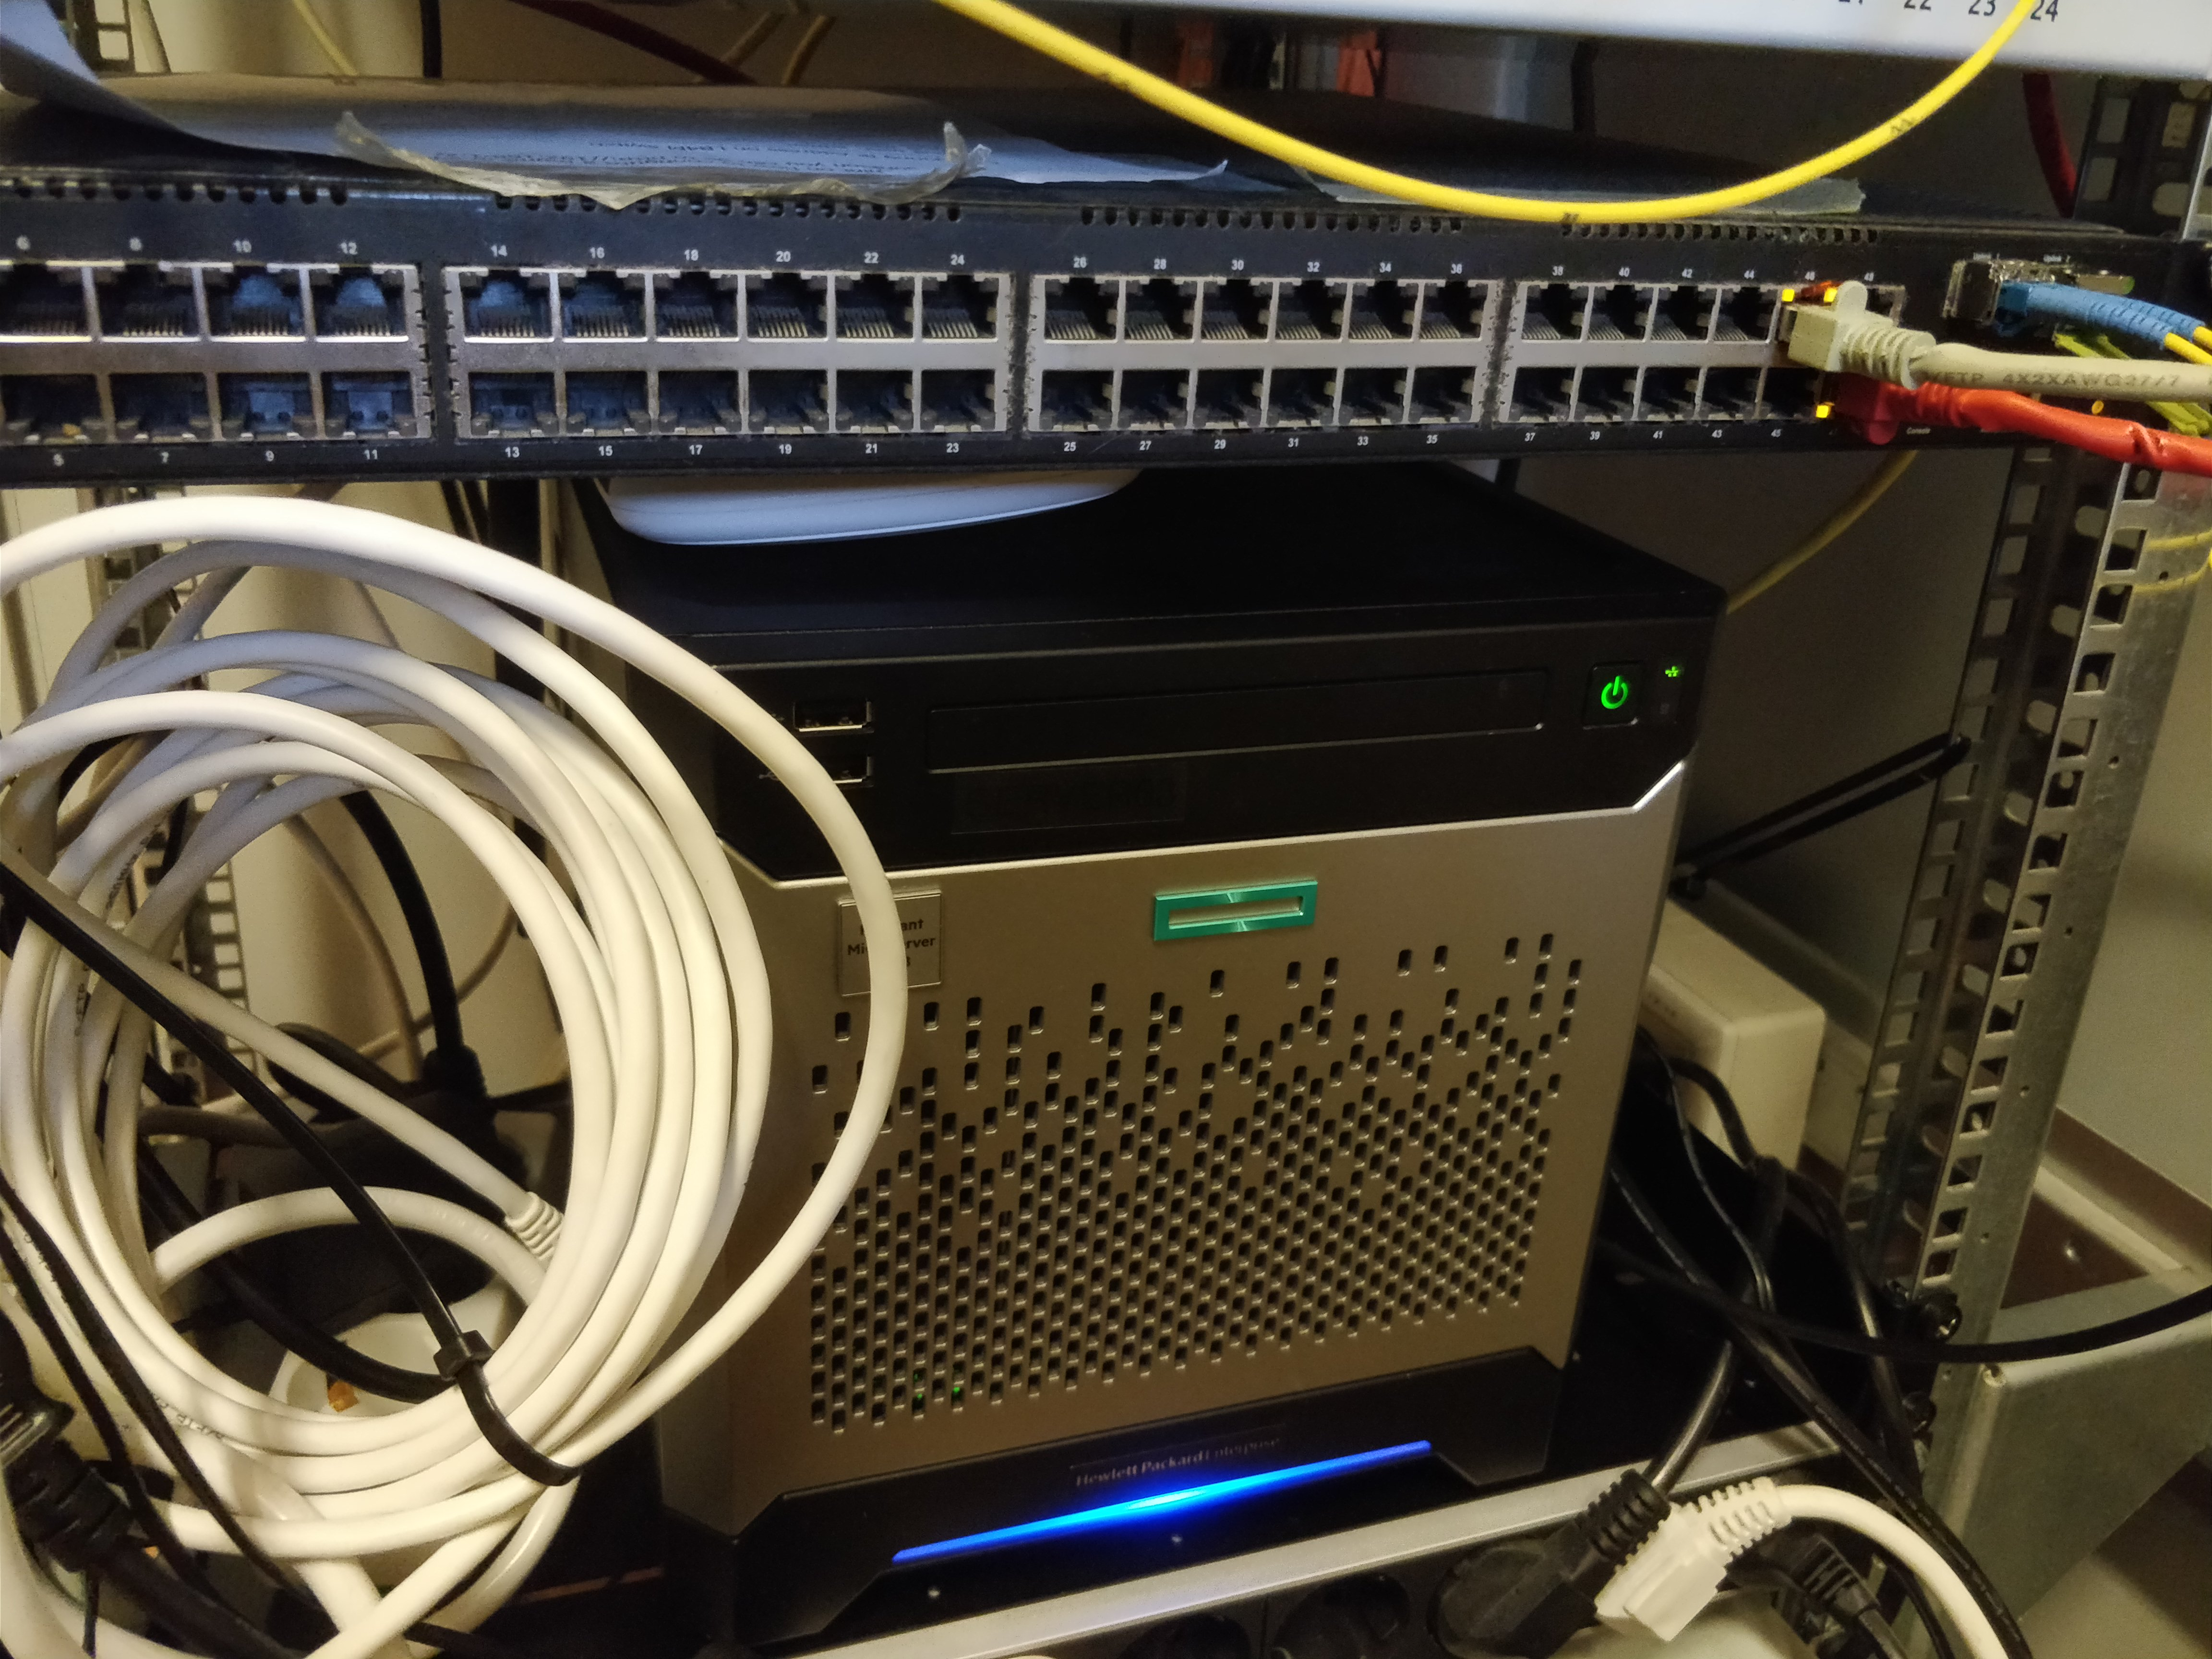
\includegraphics[width=\framewidth]{media/zbau-server.jpg}
	\end{frame}
	\begin{frame}[plain,standout]
		\centering
		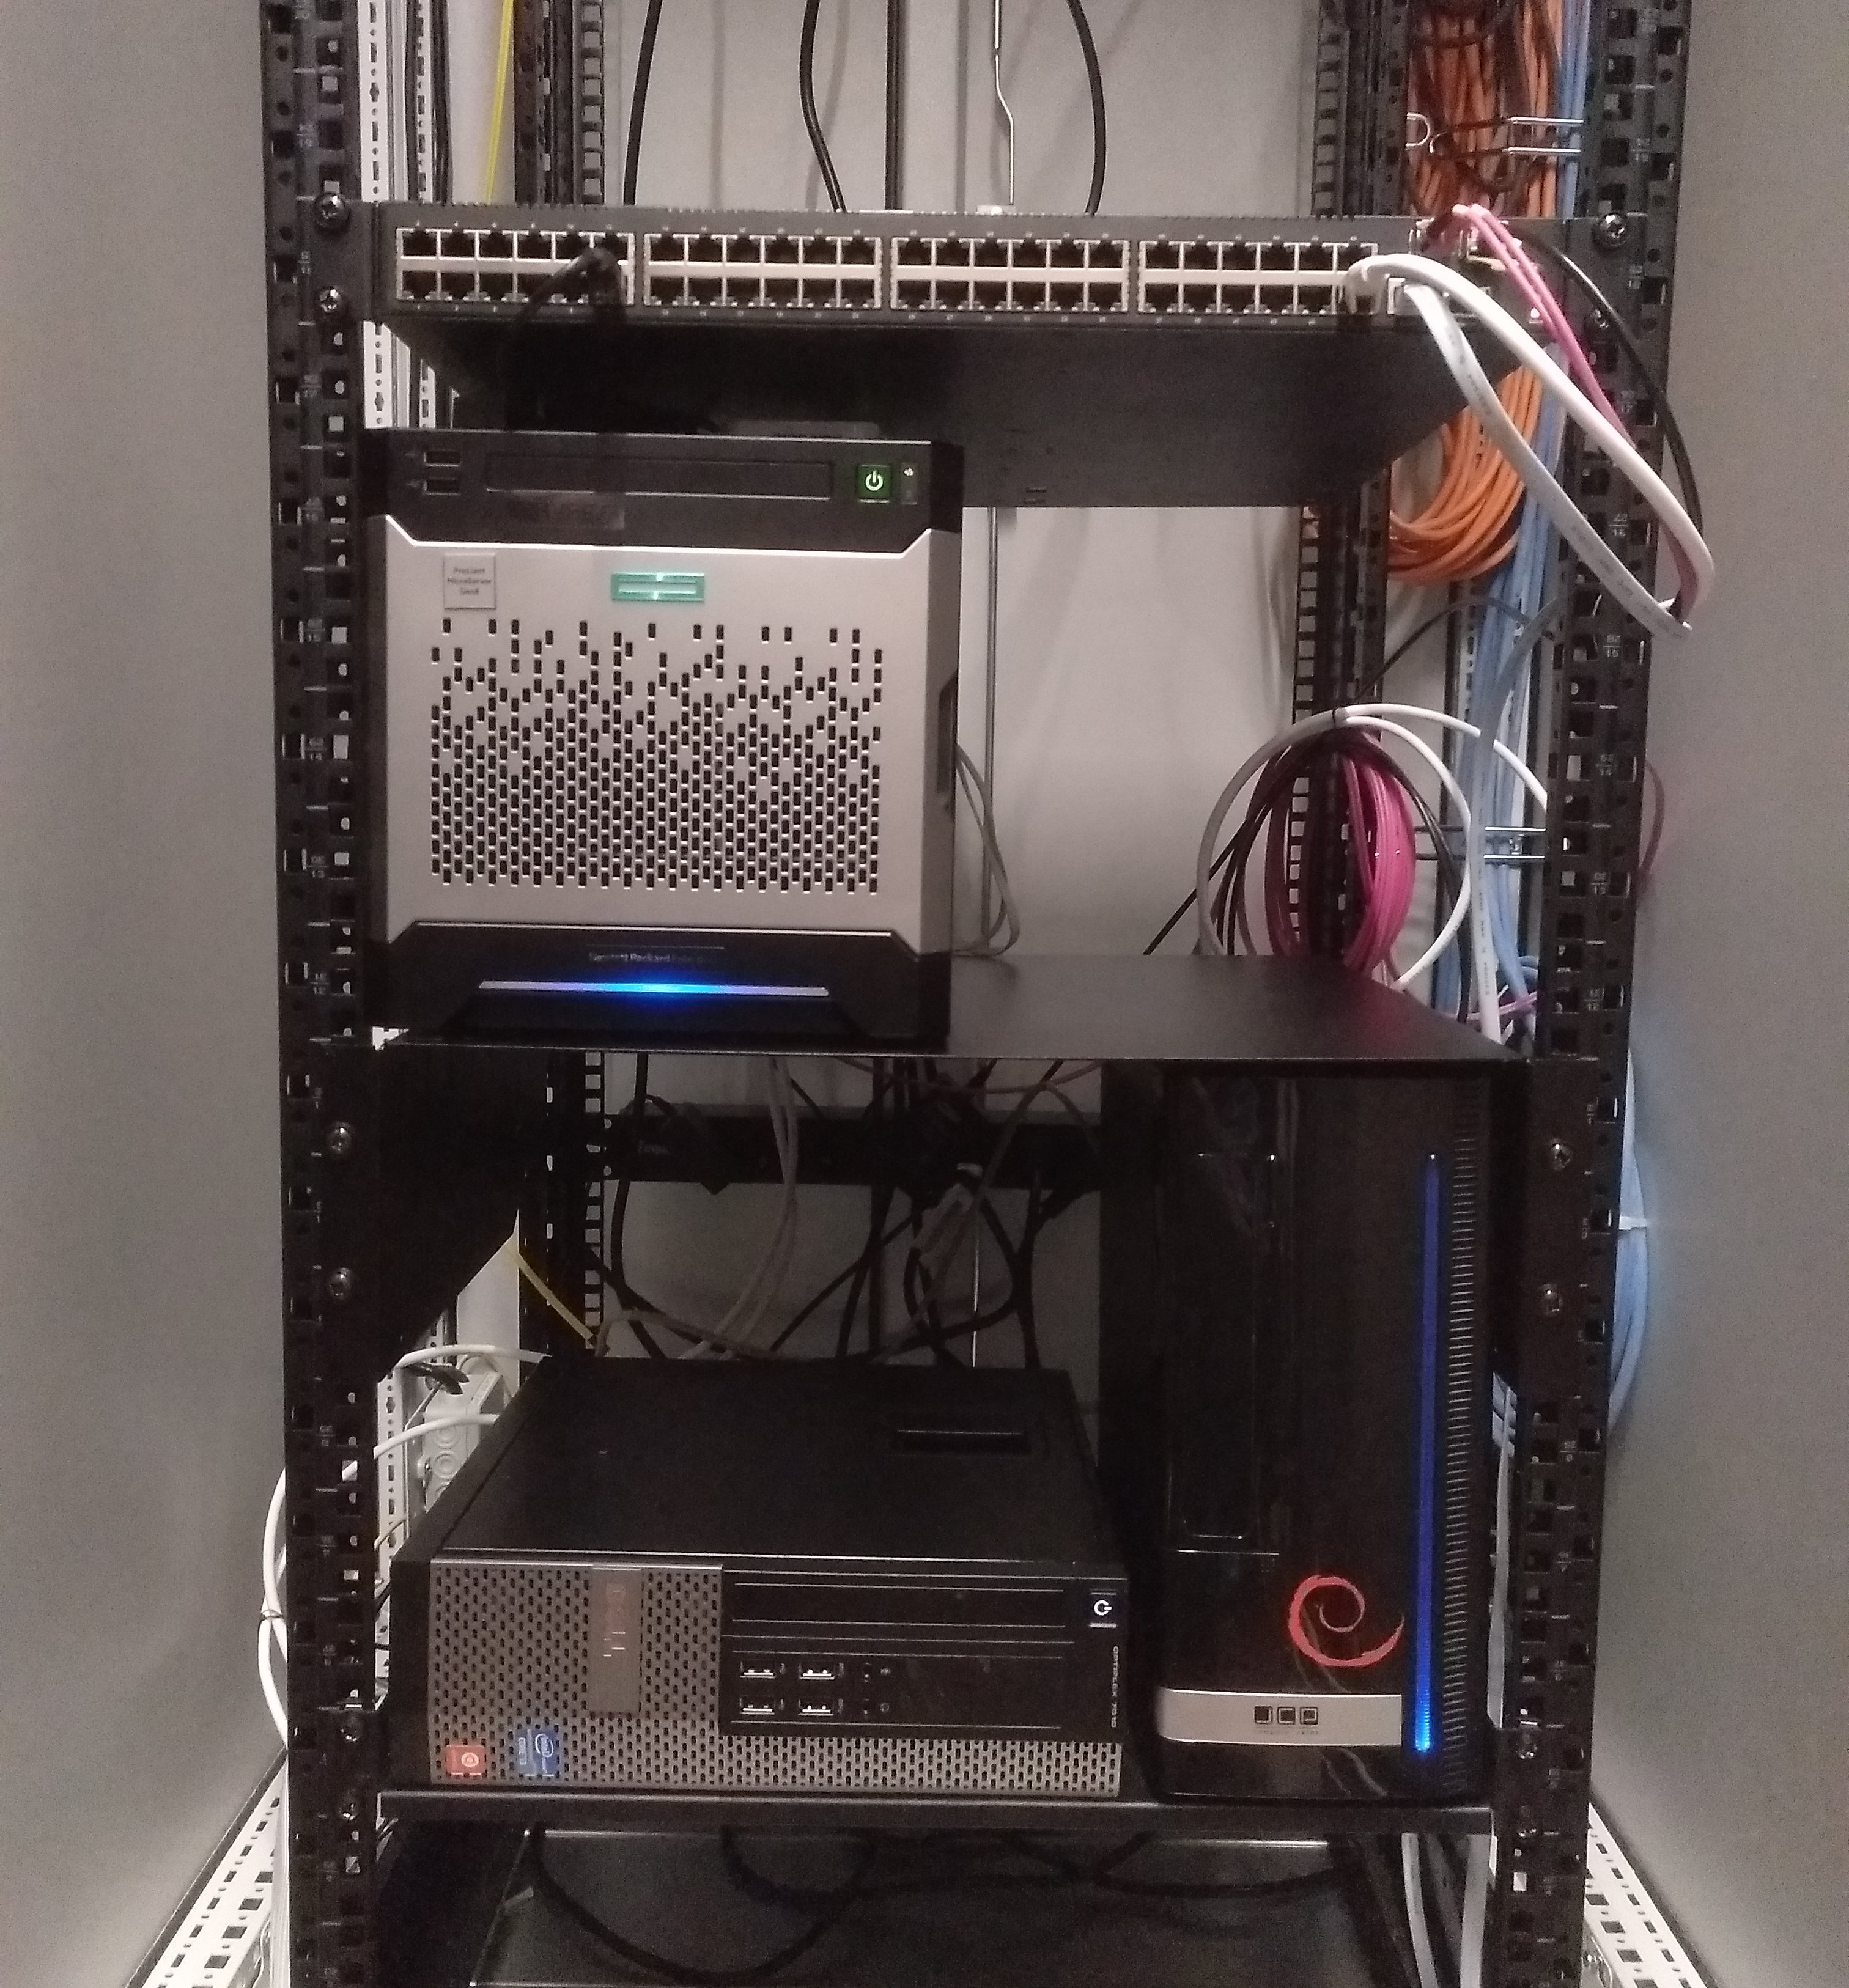
\includegraphics[height=\textheight]{media/zbau-server-neu.jpg}
	\end{frame}

% Nachteile eines gewöhnlichen Internetanschlusses [extra]
%% dynamische Adressen
%% asymmetrische Verbindung, teilweise extrem
%% Abhängig von Ausbauplänen des Providers
%% Man kann mit den Menschen Reden, die das Netz bauen
\end{document}
